%  Filename   : preamble.tex
%  Description: Preamble file to :
%               a. specify related packages
%               b. set margins, commands, etc.
%\documentclass[12pt,titlepage,onepage, letterpaper]{article}
\documentclass[12pt,titlepage,twopage, letterpaper, openany]{book}
%
%-- specify related packages
% \usepackage[utf8x]{inputenc}
\usepackage{pdfpages}
\usepackage{apacite}         %-- APA style citation  http://www.ctan.org/tex-archive/biblio/bibtex/contrib/apacite/

%no heading "References" before the references list
\makeatletter
\let\st@rtbibsection\@bibnewpage
\let\st@rtbibchapter\@bibnewpage
\makeatother

\usepackage{amsmath}       % American Math Society packages
\usepackage{amsfonts}
\usepackage{amssymb}
\usepackage{graphicx}      %needed for including figures in JPG or PNG format
 \usepackage{verbatim}     % multiple lines of comments
                               %-- example:
                               %   \begin{comment}
                               %        ...your text here...
                               %   \end{comment}
\usepackage{color}  %-- allows use of color with text
                               %-- example:  \textcolor{red}{This is the colored text in red.}
\usepackage{url}  %-- allows use of URLs example: \url{https:\ccs1.dlsu.edu.ph}
\usepackage{tabularx}
 \usepackage{setspace}
\usepackage{lineno}
\usepackage{longtable}
\usepackage{ltablex}
\usepackage{xltabular}
\usepackage{adjustbox}
\usepackage{csquotes}
\usepackage{pdflscape}
\usepackage{multicol}
\usepackage{xtab}
\usepackage{mdframed}
	
\usepackage{colortbl}
\definecolor{LightGreen}{rgb}{0.57, 0.94, 0.57}
\definecolor{LightRed}{rgb}{1, 0.61, 0.60}

%
%-- set margins,  you may need to edit this for your own printer
%
\topmargin 0.0in
\oddsidemargin 0.0in
\evensidemargin 0.0in

\voffset 0.0in
\hoffset 0.5625in

\textwidth 5.75in
\textheight 8.5in


\parskip 1em
\parindent 0.25in

% \bibliographystyle{apacite}            %-- use APA citation scheme
\hyphenation{ana-lysis know-ledge}     %-- LaTeX may not hyphenate correctly some words you use in your document
                                       %-- use \hyphenation to instruct LaTeX how to do it correctly, example above
\newcommand{\degree}{^{\circ}}         %-- use \newcommand to create your own "commands"
\newcommand{\etal}{et al.}
\newcommand{\figref}[1]{Figure \ref{#1}}
\newcommand{\appref}[1]{Appendix \ref{#1}}

%\newcommand{\Section}[1]{\section{#1}\setcounter{figure}{0}\setcounter{table}{0}}

%\newcommand{\shade}{\multicolumn{1}{|>{\columncolor[gray]{0.25}}c|}{}}
%\newcommand{\tableheader}[1]{\rowcolor{black}\color{white}{#1}}
%\newcommand{\cell}[2]{\multicolumn{1}{#1}{#2}}
%\newcommand{\definition}[2]{\textbf{\textit{#1}} --- #2}
%\newcommand{\itembit}[1]{\item \textbf{\textit{#1}}}
%\newcommand{\sgdef}[2]{\parbox[t][][t]{1.75in}{\textbf{#1}} \> \parbox[t][][t]{4.0in}{#2}\\\\}

%\newenvironment{sinagglossary}{\begin{flushleft}
%\begin{tabbing}
%\hspace{1.75in}\=\\}{\end{tabbing}\end{flushleft}}

\newcommand{\thestitle}[1]{{\Large \textsc{#1}}}


%---
%  \renewcommand{\thefigure}{\thesection.\arabic{figure}}
%  \renewcommand{\thetable}{\thesection.\arabic{table}}
%  \renewcommand{\contentsname}{Table of Contents}



%---
%  \renewcommand{\thefigure}{\thesection.\arabic{figure}}
%  \renewcommand{\thetable}{\thesection.\arabic{table}}
%  \renewcommand{\contentsname}{Table of Contents}

%   End Preamble    %

\graphicspath{{figures/}}  %figures is the name of the folder containing images JPG or PNG
\doublespacing
\begin{document}
\linenumbers
%   Filename    : title_page.tex
\begin{titlepage}
\centering

%-- **EDIT** the following line to indicate your thesis title
\thestitle{\textbf{FaKe}: Filipino Language Fake News Detection System Using Machine Learning}

\vspace{1.15cm}
A Special Problem\\
Presented to\\
the Faculty of the Division of Physical Sciences and Mathematics\\
College of Arts and Sciences\\
University of the Philippines Visayas\\
Miag-ao, Iloilo

\vspace{1.15cm}
In Partial Fulfillment\\
of the Requirements for the Degree of\\
Bachelor of Science in Computer Science
\vspace{1.15cm}
by\\

\vspace{1cm}
% list in alphabetical order by lastnames
JOCSING, Rene Andre  \\
LUPAC, Coebe Austin  \\
PONCE DE LEON, Chancy  \\
% LASTNAME4, FirstName4  \\

\vspace{1.15cm}
Francis DIMZON \\
Adviser\\
%Firstname LASTNAME \\
%Co-Adviser

\vspace{1.15cm}
\today
\end{titlepage}
      %includes LaTeX source file for the Title Page
\pagenumbering{roman}   %number pages as i, ii, iii, etc...
\setcounter{page}{2}
%   Filename    : approval.tex
\begin{center}
    \textbf{Approval Sheet}

    The Division of Physical Sciences and Mathematics, College of Arts and Sciences, University of the Philippines Visayas

    certifies that this is the approved version of the following special problem:

    \thestitle{FaKe: Filipino Language Fake News Detection System Using Machine Learning}
    \end{center}

    {\small\textbf{Approved by:}}

    \newcommand{\signaturerule}{\rule{10em}{.4pt}}
        \begin{tabular}{lll}
            \bfseries Name  & \bfseries Signature & \bfseries Date\\ \\
            Francis D. Dimzon, Ph.D. &\signaturerule  & \signaturerule\\
            \multicolumn{1}{c}{(Adviser)} \\
            Ara Abigail E. Ambita &\signaturerule &\signaturerule\\
            \multicolumn{1}{c}{(Panel Member)}  \\
            Christi Florence C. Cala-or  &\signaturerule &\signaturerule\\
            \multicolumn{1}{c}{(Panel Member)}  \\
            Arnel L. Tampos, Ph.D. &\signaturerule &\signaturerule\\
            \multicolumn{1}{c}{(Division Chair)}

        \end{tabular}

%   Filename    : declaration.tex
\begin{center}
	Division of Physical Sciences and Mathematics\\
	College of Arts and Sciences\\
	University of the Philippines Visayas

		\textbf{Declaration}
		\end{center}

We,  Rene Andre B. Jocsing, Coebe Austin V. Lupac, Chancy M. Ponce de Leon, hereby certify that this Special Problem has been written by us  and is the record of work carried out by us. Any significant borrowings have been properly acknowledged and referred.

	\begin{tabular}{lll}
	\bfseries Name  & \bfseries Signature & \bfseries Date\\ \\
	\signaturerule &\signaturerule  & \signaturerule\\
	Rene Andre B. Jocsing\\ \\
	\signaturerule &\signaturerule &\signaturerule\\
	Coebe Austin V. Lupac\\ \\
	\signaturerule &\signaturerule &\signaturerule\\
	Chancy M. Ponce de Leon
\end{tabular}

%   Filename    : dedication.tex
\begin{center}
	\textbf{Dedication}
\end{center}

``To our very own superhero.''

\begin{center}
	\textbf{Acknowledgment}
\end{center}

Throughout this study, we acknowledge the patient counsel bestowed upon us by Professor Francis D. Dimzon. His tutelage and expertise in the field of machine learning were crucial in forming the backbone of this paper.

We acknowledge the assistance rendered by Mr. Ron Gerlan F. Naragdao, in providing computational units for training the models in this study. Furthermore, his aid in designing the website for the FaKe browser extension and beta-testing the extension itself was indispensable.
%   Filename    : abstract.tex 
\begin{abstract}

    Present methods for curbing the rampant spread of misinformation in the Philippines remain inadequate. The internet used as a medium for spreading fake news necessitates fast, automated computational tools as countermeasures accessible to the public. A precursor study from 2020 benchmarks deep learning techniques in building Filipino language fake news classifiers from a low-resource dataset. Despite promising results, the models from the previous study cannot be feasibly deployed for a wide audience due to unreasonable cost of deployment. In this work, we make several contributions. First, we construct a second dataset of Filipino language news articles, alleviating resource scarcity, and name this dataset \enquote{Fake News Filipino 2024}. Next, we apply bleeding edge techniques to extract Filipino linguistic features, and use these features in training and benchmarking machine learning models. We show that robust fake news classifiers for a morphologically rich language may be constructed from simple machine learning models and a low-resource dataset. Our best model and feature space achieves an accuracy of 97\% on the corpus. Lastly, we build a cross-browser web extension for classifying Filipino language fake news using our best model. The \enquote{FaKe} web extension has been made available to the public on this paper's code repository.
    
    \begin{comment}
        Finalize abstract once tuned results from Chip are in.
    \end{comment}
    
    %  Do not put citations or quotes in the abstract.
    
    \begin{flushleft}
    \begin{tabular}{lp{4.25in}}
    \hspace{-0.5em}\textbf{Keywords:}\hspace{0.25em} & machine learning, natural language processing, fake news, journalism, computers in other domains, filipino language, filipino linguistic features, classifiers, feature extraction, hyperparameter tuning, low-resource dataset, naive bayes, logistic regression, random forest, svc
    \end{tabular}
    \end{flushleft}
    \end{abstract}
    
            %includes the the Abstract page
\tableofcontents                  %generate the Table of Contents
\newpage
\listoffigures                    %generate List of Figures
\newpage
\listoftables                     %generate List of Tables
\newpage
\pagenumbering{arabic}            %number pages as 1, 2, 3, etc...
\setcounter{page}{1}
%\linenumbers
%   Filename    : chapter_1.tex
\chapter{Introduction}
\label{sec:researchdesc}    %labels help you reference sections of your document

\section{Overview}
\label{sec:overview}

A type of propaganda or \textit{yellow journalism}, fake news \cite{nyt-trump-lies} can be categorized as deliberate misinformation spread via print media, broadcast media, or online media. The rampant rise of fake news propagated over the internet and social media has become a cause for concern.

According to the World Economic Forum \cite{weforum-report}, misinformation ranks among the world's top global risks as fake news outlets see astounding traffic and engagement. An economic analysis by Israel-based cybersecurity firm CHEQ and the University of Baltimore \cite{pids-report} reveals that fake news costs the global economy a baffling 78 billion USD. A survey from Social Weather Stations (SWS) \cite{juan-felix-et-al-2023} reports that 51\% of Filipinos find it difficult to spot fake news. Journalists and political analysts speculate that Philippine former President Rodrigo Duterte's landslide victory in the 2016 presidential elections has been largely brought about by paid trolls disseminating fake news articles through social media outlets \cite{harvard-cyber-report}. During the 2016 elections, Duterte popularizes a depiction of the Philippines as a \enquote{\textit{narco-state}}\cite{demick2016duterte}. He earns tremendous publicity through his narco-state rhetoric, justifying more than 7,000 extra-judicial killings \cite{alconaba2016digong} and gaining enough notoriety to sway the voters to his corner. Despite Duterte's insistence that his rhetoric is the truth, the United Office on Drugs and Crime claims otherwise—the Philippines' drug use prevalence is lower than the global average \cite{yee2017posttruth}.

A number of institutions have devised several strategies to combat fake news. These strategies can be broadly categorized into four primary areas: the language approach, the knowledge-based approach, the machine learning approach, and the hybrid approach \cite{debeer2020approaches}.

In the language approach, a human or software inspects linguistic structure to identify fake news through grammar and syntax \cite{burkhardt2017history}. Authors of fake news often have great control over its contents, but they can be identified through their style of writing \cite{yang2018ti-cnn}. The language approach also entails bag of words (BOW), semantic analysis, and deep syntax. The BOW method assumes independence and importance of each word in a paragraph \cite{burkhardt2017history}. Analysis of word frequencies (also called \textit{n}-grams) is carried out to identify misinformation \cite{thota2018fake}. However, the BOW method does not take context into consideration, so its practicality is limited \cite{potthast2017stylometric}. Semantic analysis involves the determination of truthfulness through the comparison of personal experience to a profile derived from related articles, based on the premise that honest writers are more likely to make similar remarks about a topic \cite{chen2015news}. Deep syntax exploits probabilistic context free grammars to transform sentences into a set of rules used in analyzing a piece of text, which may lead to patterns that ultimately discern between truth and lies \cite{zhou2020survey, Stahl2018FakeND}.

The knowledge-based approach requires a myriad of fact-checking techniques to identify fake news. However, this approach is challenged by fake news spreading swiftly and unchecked through social media platforms \cite{qazvinian2011rumor}, which necessitates some form of automation in detecting fake news. Knowledge-based approaches can be further categorized into expert oriented fact checking, computational oriented fact checking, and crowdsourcing \cite{debeer2020approaches}. Expert oriented fact checking employs professionals in verifying the accuracy of a particular claim through manual research, comparing text to another which has been previously fact-checked \cite{vlachos2014factchecking}. The computational based approach leverages automated fact checking tools in determining the authenticity of news \cite{ahmed2019combining}. A tool named ClaimBuster \cite{claimbuster, hassan2017proposal} has been developed to automate the identification of English language fake news through machine learning and natural language processing \cite{hassan2017toward}. It requires a database of known facts to compare context with social media posts, interviews, and speeches in real time, delivering results to the user \cite{hassan2017toward}. Crowdsourcing approach, on the other hand, relies on the wisdom of the crowd in determining the authenticity of a claim \cite{ahmed2019combining}. The accuracy of news is measured through the collective decision of the crowd \cite{pennycook2019fighting}. An example of a platform that enables the crowdsourcing approach is Facebook \cite{tschiatschek2017detecting}. In 2017, the National Union of Journalists in the Philippines (NUJP) releases Fakeblok, a Chrome web extension that blocks articles by known fake news publishers from appearing on a user's Facebook feed \cite{inquirer-fakeblok, rappler-fakeblok}. These websites tagged as fake news publishers are collected in a database maintained by the NUJP. A website may be reported by users as fraudulent. Once reported, a team of expert Filipino journalists scrutinizes the website. If found fraudulent, it is added to the database \cite{cdi-fakeblok}. However, as of the time of writing, the Fakeblok extension can no longer be found on the Chrome web store, rendering it unavailable to the public.

In the machine learning approach, datasets are used to train models in identifying fake news \cite{debeer2020approaches}. Machine learning models may be used to automate fake news detection. Datasets may be constructed through crowdsourcing \cite{perezrosas2018automatic} or webscraping \cite{cruz2020localization}. Twitter implements a machine learning powered approach called the rumor identification framework, where the metadata of tweets is processed to alert users if a tweet may be false \cite{sivasangari2018modern}. The Twitter crawler has also been developed by Twitter, a machine learning powered system that collates tweets into a database, making comparisons feasible \cite{atodiresei2018identifying}. Recent studies advocate for the hybrid approach \cite{debeer2020approaches}, integrating human knowledge engineering with the machine learning approach in identifying fake news \cite{ruchansky2017csi, okoro2018hybrid}. However, this paper turns its lens exclusively on the machine learning approach in tackling the identification of Filipino language fake news. The classification of fake news is treated as a computer science problem.

\section{Problem Statement}

In the past decade, machine learning models have made
great strides in distinguishing between fake and authentic news articles \cite{ahmed2021detecting}. Fake news via false or sensational claims are being identified by Facebook, Twitter, and Instagram through machine learning models \cite{debeer2020approaches}. Machine learning models enable a system to intelligently analyze patterns from data, with no specific programming. They can be grouped into four major categories: supervised, unsupervised, semi-supervised, and reinforcement \cite{sarker2021machine}.

Deep learning models, on the other hand, are a subset of machine learning models that utilize a computational architecture (neural network) comprised of multiple input, output, and hidden layers to process data \cite{sarker2021machine}. The performance between the two types of model varies, with deep learning generally performing better on large datasets \cite{xin2018machine, sarker2020cybersecurity}.

A study by \citeA{khan-2021} benchmarks multiple machine learning and deep learning models in classifying English language fake news. They use a dataset containing English language news articles written about a vast array of topics ranging from politics, sports, and entertainment. Their results suggest that detecting English language fake news using machine learning models yields favorable outcomes, with Naïve Bayes achieving a 93\% accuracy on their joint corpus. However, their study utilizes a relatively large dataset containing 80,000 news articles written in English. Unfortunately, as of the time of writing, no such dataset exists for news articles in the Filipino language.

To begin filling this gap, \citeA{cruz2020localization} pioneer the first low-resource Filipino language news dataset with 3,206 expertly labeled articles. They benchmark various machine learning techniques to train robust fake news classifiers from a relatively small amount of data. Despite their promising results, the models that they investigate cannot be easily deployed for consumer-level applications, thus having a limited audience \citeA{cruz2020localization}. The deployment of Bidirectional Encoder Representations from Transformers (BERT), a state-of-the-art deep learning model used in Cruz's study, costs anywhere from 50,000 USD to 1,600,000 USD \cite{paleyes-2022} depending on the size of the model. This cost of deployment is unreasonable for institutions and companies. Therefore, we investigate lightweight machine learning models that may provide adequate performance in distinguishing between fake and authentic Filipino language news articles.

\section{Research Objectives}
\label{sec:researchobjectives}

\subsection{General Objective}
\label{sec:generalobjective}

We investigate machine learning models that may provide adequate performance in distinguishing between fake and authentic Filipino language news articles. To this end, we construct a dataset of Filipino language news articles, named Fake News Filipino 2024, to augment Fake News Filipino \cite{fake-news-filipino}. We build a third dataset, a joint corpus that combines the two datasets. In training the models, we extract Filipino linguistic features \cite{imperial-2020, imperial-2021} through natural language processing techniques. We perform hyperparameter tuning and benchmark the performance of these classifiers across the three datasets. Lastly, we deploy the most suitable model as a cross-browser web extension for classifying Filipino language fake news articles.

\subsection{Specific Objectives}
\label{sec:specificobjectives}

Specifically, we:

\begin{enumerate}
   \item Source Filipino language news articles from the web and build a balanced dataset of fake and authentic news articles;
   \item Extract Filipino linguistic features from a corpus of multi-domain Filipino language news articles;
   \item Train machine learning models in classifying fake Filipino language news articles through Filipino linguistic features;
   \item Benchmark machine learning models, performing hyperparameter tuning, across three different datasets; and
   \item Deploy the most suitable model as a web service and minimize cost of deployment;
\end{enumerate}

\section{Scope and Limitations of the Research}
\label{sec:scopelimitations}

In this study, we investigate machine learning models, excluding pre-trained and deep learning models. We limit our study to news articles and exclude other forms of fake news such as spam and tweets. We constrain the machine learning models in the study to a low-resource dataset, Fake News Filipino \cite{fake-news-filipino}, augmented by a similar dataset of our own, Fake News Filipino 2024. Adhering to the dataset construction methodology presented by \citeA{cruz2020localization}, Filipino language news articles are sourced from the internet via webscraping. Authentic news articles are sourced from mainstream Filipino language news websites like The Philippine Star and ABS-CBN. Fake news articles are sourced from fraudulent online sites tagged by non-profit independent fact-checking organizations such as VERA Files and the NUJP. Accuracy and model size are used as primary metrics for ranking the performance of the models. We deploy the most suitable model in an application system. The application system is constrained to a user-script on the client-side and a web service running on a cloud server. We utilize Tampermonkey (a cross-browser extension manager) and Render (a platform as a service vendor with a free-forever tier) in deploying the application system to minimize cost of deployment.

\section{Significance of the Research}
\label{sec:significance}

Our study is significant to the field of machine learning and fake news detection due to the following reasons.

Building on the work of \citeA{cruz2020localization}, our study contributes to the field of machine learning and computer science by investigating possible machine learning models that can distinguish between fake and authentic Filipino language news articles. We offer a more extensive and diverse collection of news articles by building a dataset similar to Fake News Filipino \cite{fake-news-filipino}. Our approach not only enhances the robustness of potential models in this study, but also provides a more comprehensive dataset that may be utilized in future research.

Furthermore, we provide a lightweight application system for the Filipino audience to aid them in fact-checking and avoiding harm caused by fake news. We pave the way for the low-cost deployment of fake news classifiers to the benefit of various institutions, particularly those engaged in tagging websites that publish fake news. The exploration of low-cost machine learning deployment strategies is beneficial for computer scientists aiming to implement machine learning models in resource-constrained contexts. Our results could further the development of cost-effective solutions when deploying machine learning models in various settings.

For policymakers, our study provides them with leverage in informing and shaping policies congruent to information integrity. The low-cost deployment of effective fake news detection classifiers may be integrated into broader strategies aimed at preventing the spread of misinformation and maintaining a trustworthy Filipino news network. The deployment of a lightweight application system for fake news detection may serve as a practical tool for policymakers to empower the public in distinguishing between fake and authentic news. We dedicate our efforts in this study to promoting media literacy and arming individuals with an accessible fact-checking tool to combat fake news effectively.
               %LaTeX source file for Chapter 1: Introduction
%   Filename    : chapter_2.tex 
\chapter{Review of Related Literature}
\label{sec:relatedlit}

In this section, we synthesize relevant information gathered from other related studies relating to machine learning models in the domain of natural language processing and fake news detection.

\section{ML in Automating Fake News Detection}

Machine learning models can be used in automating the detection of fake news. \citeA{khan-2021} benchmarks multiple machine learning methods for online fake news detection. They evaluate the models on three diverse datasets, using deep learning and pre-trained models alongside traditional ones. Their results indicate that Naive Bayes with n-gram performs the best out of all the traditional models, scoring a 93\% accuracy on the combined corpus. In Naive Bayes, the addition of sentiment and lexical features does not provide a significant increase in performance. However, with sentiment and lexical features, Support Vector Machine (SVM) and Logistic Regression models outperform other traditional machine learning models except for Naive Bayes at 72\% and 77\% accuracy respectively.

Naive Bayes models are simple probabilistic classifiers that apply Bayes' theorem, assuming strong independence between the features of the dataset (naive). \citeA{granik-2017} train a Naive Bayes classifier on articles sourced by Buzzfeed from Facebook. They achieve an accuracy of 75.40\% with their Naive Bayes classifier on the dataset. Their study is limited by the size of their dataset with only 2,000 articles. Furthermore, the articles in the dataset were not of significant length and were often merely previews to a lengthier news article. They also fail to take into account stop-words and rarely used words. Lastly, they do not perform stemming on their dataset. \citeA{krishna-2021} also delves into the application of Naive Bayes in fake news detection. They benchmark Multinomial Naive Bayes classifiers on a labeled dataset comprised of fake and authentic news articles. They perform stemming and pre-processing on the dataset before training. Their results show that Naive Bayes with Term Frequency-Inverter Document Frequency (TD-IF) vectorizer scores an 85.7\% accuracy. With a count vectorizer, it scores an 89.3\% while with a hashing vectorizer, it scores 90.2\%. \citeA{krishna-2021} show that even a simple machine learning model such as Naive Bayes can perform well in detecting fake news. The features that they use in their study are N-count of the most used words, and-or phrases, casing, and stop-words such as \enquote{the} and \enquote{a}. However, their study fails to take other lexical features into account.

\citeA{tiwari-2020} train multiple ML classifiers on a dataset of real and fake news gathered from online sources, with a 50-50 split. They also utilize a count vectorizer, a TF-IDF vectorizer, and a hashing vectorizer similar to the study of \citeA{krishna-2021}. They compare numerous classifiers on the dataset. Logistic Regression performs the best with TF-IDF vectorizer, achieving a 71\% accuracy. \citeA{choudhury-2022} uses TF-IDF vectorizer to select features in their study. They compare SVM, Naive Bayes, Logistic Regression, and Random Forest models on three diverse datasets. They report that SVM attains the highest accuracy at 96\% on the aforementioned dataset, followed by a 95\% accuracy with Random Forest and Logistic Regression. Naive Bayes performs worse at only 90\% accuracy. However, the Fake News dataset is relatively large with around 20,000 English news articles. For low-resource languages like Filipino and with a small dataset, these classifiers may perform differently.

\section{Pre-processing and Feature Engineering}

\citeA{cruz2020localization} pre-process their dataset lightly to retain information such as capitalization, punctuation, and misspelled words. Pre-processing of the text is required to clean and analyze a dataset. The dataset they use in their study, Fake News Filipino, is primarily in Filipino, with the addition of borrowed English words.  They use a Moses Tokenizer to derive descriptives from the dataset. In their data pre-processing, \citeA{cruz2020localization} only perform Byte-Pair Encoding (BPE) for tokenization. BPE is used as it allows their models to represent out-of-vocabulary (OOV) words. Additionally, BPE treats morphemes as the smallest token forms instead of whole words. Thus, it is useful for models in training classifiers for morphologically-rich languages.

\citeA{fernandez-2019} highlight 76 relevant linguistic features in identifying English language fake news in the Filipino context, sorted into 8 categories. These 8 categories are readability scores, linguistic dimensions, summative cues, affective cues, informality cues, cognitive cues, punctuation cues, and time-orientation cues. Features that do not require dictionaries such as readability scores, word count, syllables count, and words per sentence are implemented in Python using regular expressions and the Natural Language Toolkit. They extract dictionary-based features from The Linguistic Inquiry and Word Count software by \citeA{pennebaker-2007}. Of the seventy-six linguistic features, the top ten features with the highest mutual information scores are headline syllables count, headline word count, headline words per sentence, content present focus, headline difficult words count, headline function words, content difficult words count, and headline prepositions. \citeA{fernandez-2019} conclude that fake and authentic news differ significantly in terms of word count, sentence count, verb tenses, and readability scores. However, despite their corpus being in the Filipino context, the articles within are written in the English language. The relevant linguistic features for identifying Filipino language fake news may differ.

In a similar vein, a study by \citeA{fayaz-2022} list a total of 23 features extracted from the ISOT Fake news data set. All features are not equally important. Some features contribute positively to model accuracy, while the others negatively impact model performance. The authors reduce the feature space to 14 features using chi\textsuperscript{2}, univariate, feature importance, and information gain. Common features among the four selection techniques include word count, number of uppercase and lowercase characters, character count, sentence count, readability scores and indices, and TF-IDF.

However, the technology to extract these advanced linguistic features from Filipino text has been slow to develop, presenting a gap in the field of natural language processing. Specifically, popular metrics for readability scores are tailored for English texts and are not appropriate for Filipino texts. As of the time of writing, no standardized instrument or assessment tool exists for measuring the readability of texts in the Filipino language \cite{imperial-2020}. However, initial forays into this gap are promising. \citeA{Macahilig2015ACR} developed a formula for assessing the readability of modern Filipino texts, wherein readability score is a function of word count and words per sentence. \citeA{imperial-2020} and \citeA{imperial-2021} (two separate studies conducted by the same authors) present different linguistic feature sets in measuring Filipino text readability. They compare the different combinations of traditional features, lexical features, and language model features in measuring Filipino text readability. Using linear regression with the combination of all 25 predictors from the three feature sets produces the highest evaluation score of 72.0\%. Using Spearman correlation and information gain, they identify polysyllable word count, word count, sentence count, and average sentence length as the top predictors for the traditional features. For the language model features, the top predictors are all the three trigram models trained for the model. No predictor from the lexical features has been identified as a top predictor, which may imply that lexical features alone cannot be used for Filipino readability measurement. In addition to traditional, lexical, and language models, the authors append syllable patterns and morphological features to the feature space \cite{imperial-2021, imperial-2020}. As of the time of writing, no study implements these Filipino linguistic features in training ML models for the purpose of Filipino language fake news detection.

\section{Summary}

The established literature bares a lack of investigation into machine learning algorithms in the domain of Filipino language fake news. Linguistic features and readability metrics for Filipino texts are also in a stage of infancy. At the present, a large dataset for Filipino language news articles does not exist. Despite these setbacks, \citeA{cruz2020localization} train deep learning models in classifying Filipino language fake news on a low-resource dataset. However, the models they train cannot be feasibly deployed in a fake news detection system due to unreasonable cost of deployment \cite{paleyes-2022}. Application of Filipino linguistic features highlighted in \citeA{imperial-2020} and \citeA{imperial-2021} has not been explored in training Filipino language fake news classifiers. In summary, while English language fake news classifiers and English linguistic features are well-trodden ground, the same cannot be said for their Filipino counterparts.

\begin{comment}
\end{comment}               %LaTeX source file for Chapter 2: Review of Related Literature
%   Filename    : chapter_3.tex
\chapter{Research Methodology}

The steps outlined in the following sections were conducted.

\section{Data Gathering}

Filipino language news articles, both fake and authentic, were sourced from the internet.

Specifically, the data-gathering methodology outlined in the work of \cite{cruz2020localization} was adapted to refrain from reinventing the wheel and to ensure consistency between fresh and old data. To augment the Fake News Filipino dataset from their study with a similar dataset, fake news articles were sourced via web scraping from various fraudulent websites tagged by VERA Files. As an independent non-profit organization in the Philippines, its mission is to engage in extensive research and the writing and production of media, in pursuit of excellent journalism \cite{verafiles-about}. VERA Files boasts several fact-checking ventures, including VERA Files Fact Check \cite{verafiles-fact-check}. On the other hand, authentic news articles were sourced from trusted mainstream providers such as The Philippine Star and ABS-CBN. Python's \textit{BeautifulSoup4} and \textit{selenium} libraries were utilized in the development of the article scraper. The articles and the corpus were encoded in UTF-8. Minimal preprocessing of the text was conducted to preserve features such as misspelled words and incorrect punctuation. The news articles were mostly Filipino with a few words in the English vernacular. Scraped fake news and authentic news were labeled accordingly as Fake (0) or Real (1).

\section{Model Training and Data Processing}
\label{sec:ModelTraining}

Figure \ref{fig:Model} shows the steps in model training and data processing. The text input were tokenized, the features were extracted, and the models were trained using the extracted features.

The corpus was tokenized using a pre-trained BPE tokenizer from \citeA{cruz2020localization}. Linguistic features highlighted by \citeA{fernandez-2019} as well as \citeA{fayaz-2022} were used in training the models. Table \ref{tab::Features} describes the features to be extracted and specifies their predictors. These features include traditional or surface-based features such as word count, sentence count, and character count. These features were extracted via a library of Python scripts designed specifically for the extraction of Filipino linguistic features \cite{imperial-2020, imperial-2021}. Through the same library, syllabic features based on the prescribed Philippine orthography, lexical features such as type-token ratio, and morphological features such as morphemes were extracted. Additionally, the misspelled word frequency, out-of-vocabulary (OOV) word frequency, stop words frequency, and the readability formula for modern Filipino texts developed by \citeA{Macahilig2015ACR}, which has not been investigated as a linguistic feature of Filipino texts in previous studies, were appended to the feature space. The tokens were vectorized with TF-IDF, extracting unigrams, bigrams, and trigrams as well as bag-of-words. The following classifiers were trained using the extracted features: Multinomial Naive Bayes, Logistic Regression, Random Forest, and Support Vector Classifier (SVC).

\begin{figure}[h]
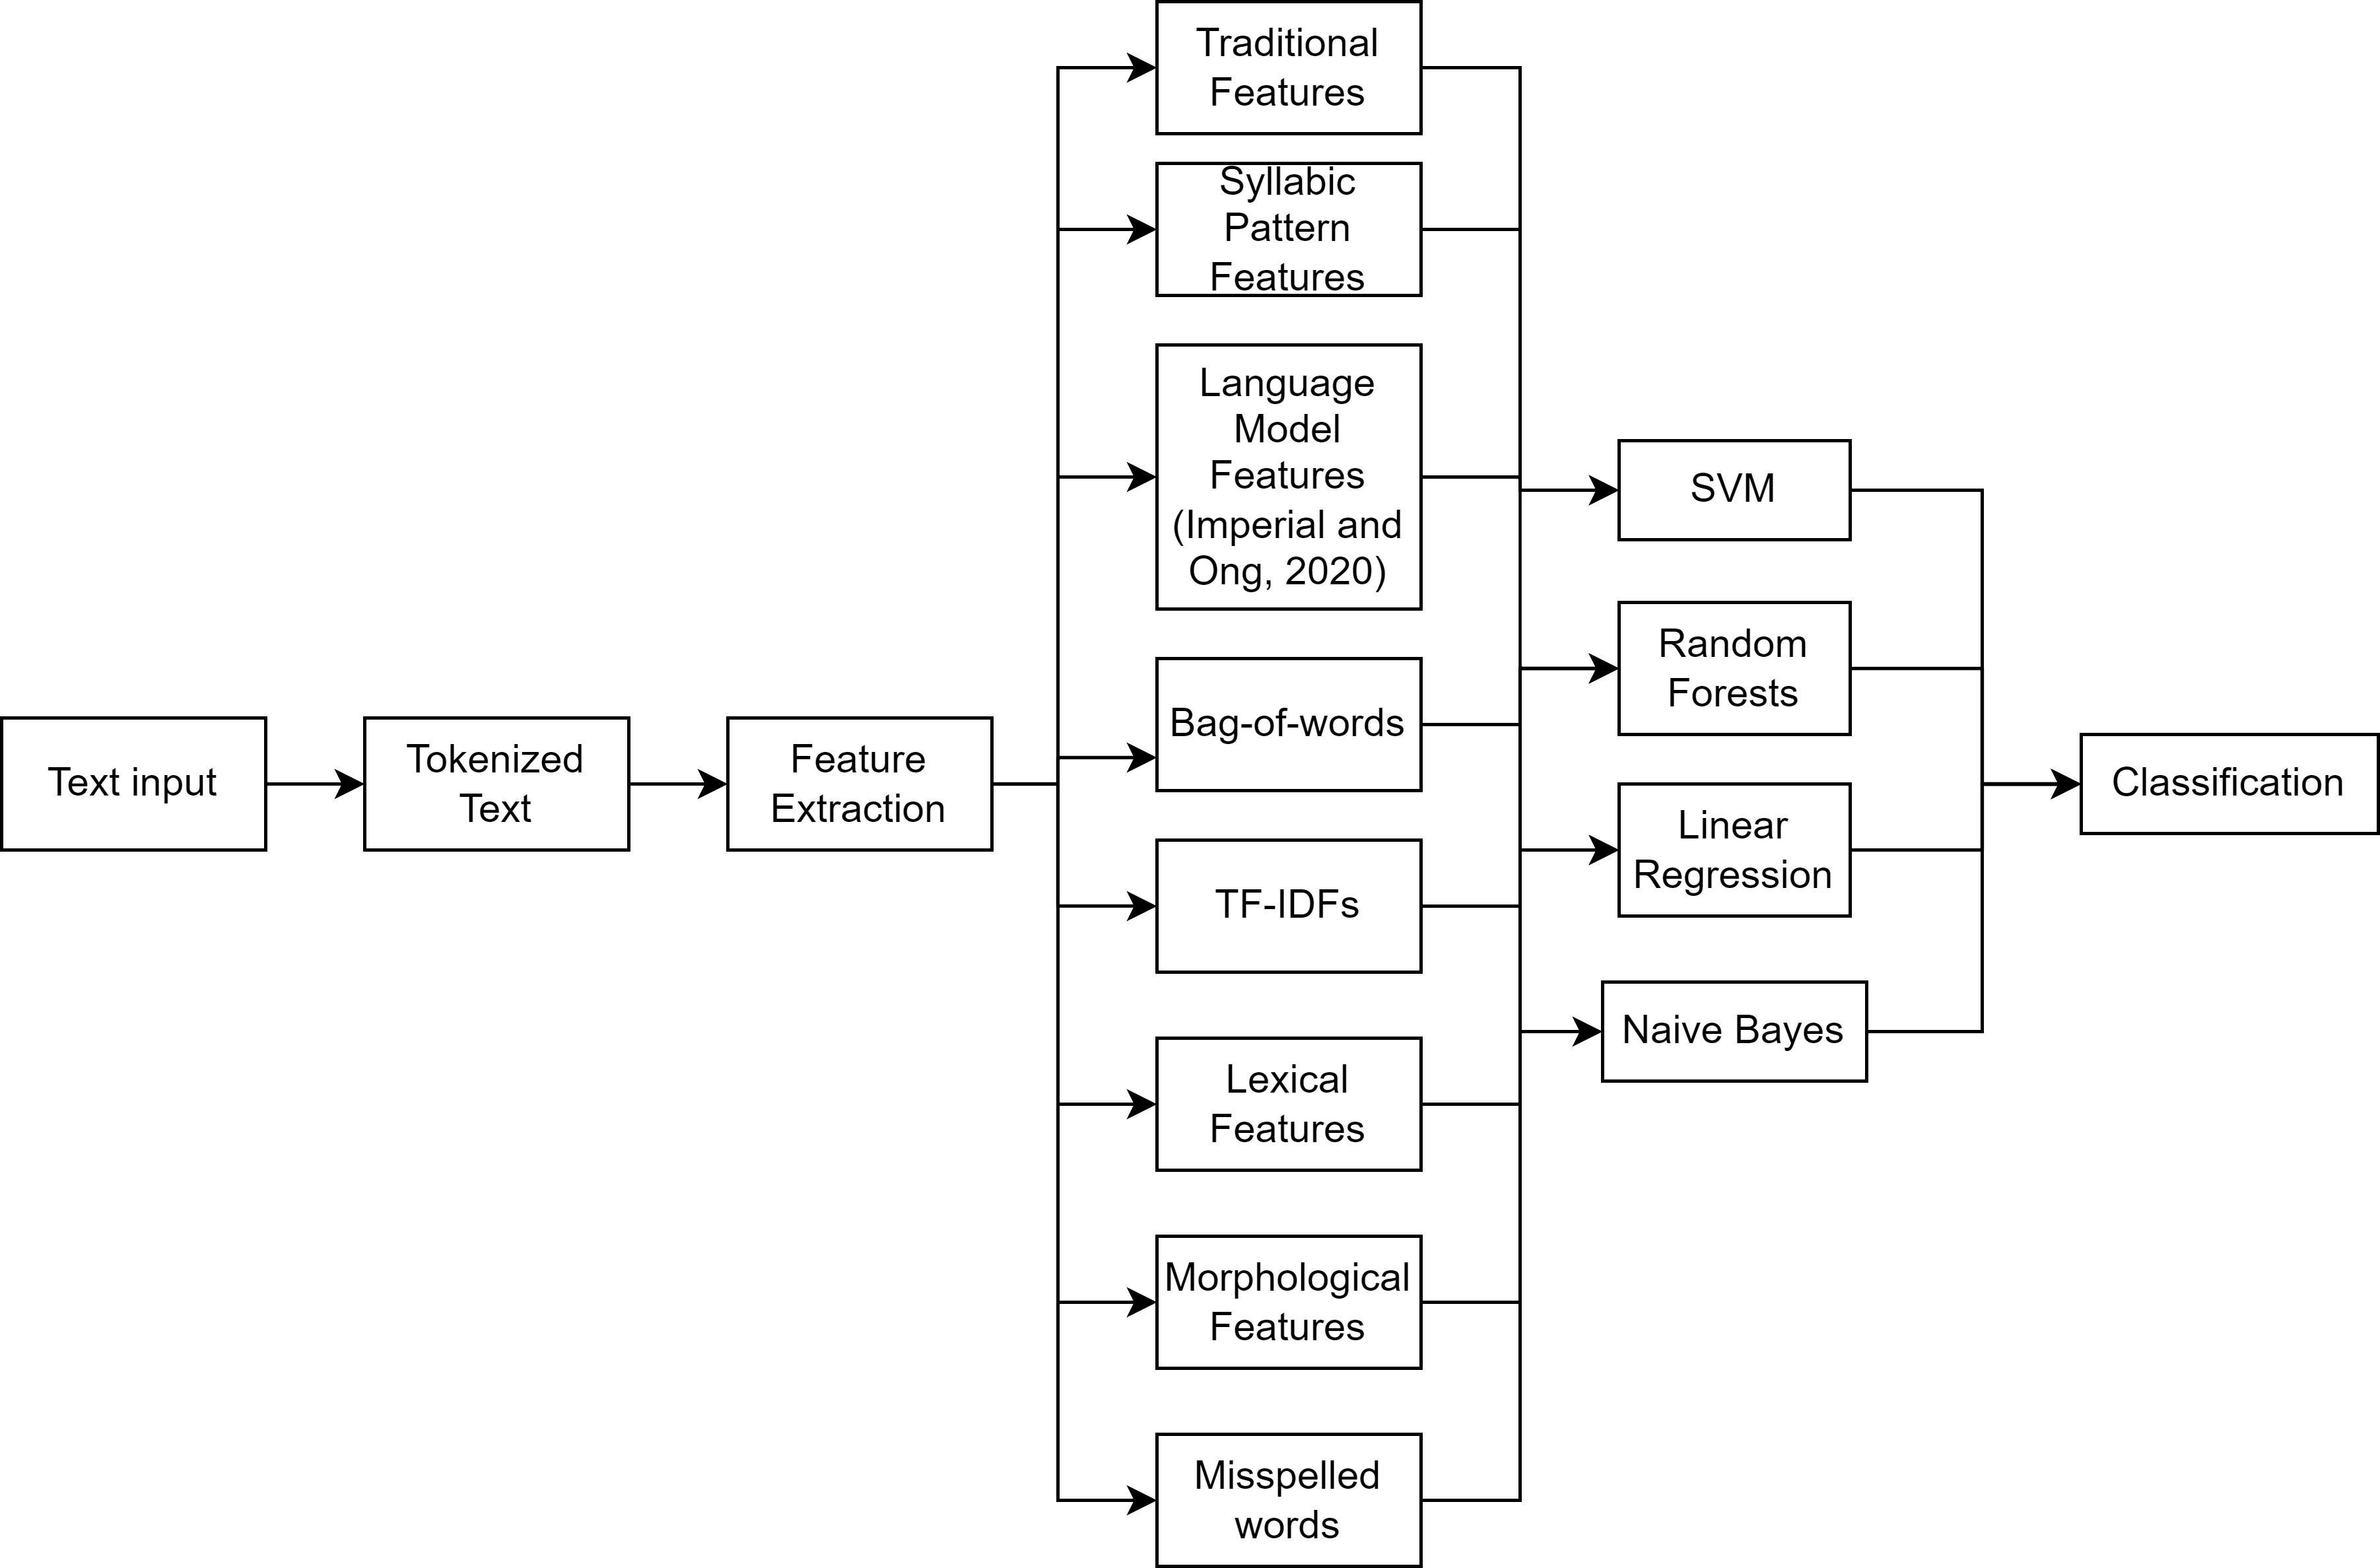
\includegraphics[width=\textwidth,height=\textheight,keepaspectratio]{figures/Model Training.png}
  \caption{Data Processing and Model Training}
  \label{fig:Model}
\end{figure}

\clearpage

\begin{tabularx}{\textwidth}{|X|X|X|}
     \hline Feature & Description & Predictors \\ \hline
     \endfirsthead

     \hline
     \multicolumn{3}{|r|}
     {Continued from previous page.} \\
     \hline
     Feature & Description & Predictors \\ \hline
     \endhead

     \hline \multicolumn{3}{|r|}{{Continued on next page...}} \\ \hline
     \endfoot

     \hline
     \caption{Descriptions and predictors of features.}
     \endlastfoot

     Bag-of-words & Unordered collection of words. & Bag-of-words model of the input text. \\
     \hline
     TF-IDF & Word to document ratio in the corpus. & TF-IDF using n-gram values of \{ 1, 2, 3\}. \\
     \hline
     Misspelled words & Misspelled words in the input text. & Total misspelled word count. \\
     \hline

    OOV words & Words in the input text that are not found in the Filipino and English dictionary used in training & Total OOV word count. \\
    \hline
    Stop words & words considered insignificant in processing text input e.g. "at", "ay", "din", etc. in Filipino or "a", "the", "to", "as" in English. & Total stop word count. \\
    \hline
    Filipino readability formula & Readability formula for Filipino text by \citeA{Macahilig2015ACR}. The higher the readability index, the more difficult the text is to read. & Readability is computed by: \( P = -4.161 + 0.280(w/s) + 0.106(cw)\) where P is the readability index, w/s is the average number of words per sentence, and cw is the word count. \\
    \hline
     Traditional & Traditional or Surface-based features based on counts and frequencies & Total word, sentence, phrase, polysyllabic word counts. Average word length, sentence length, syllable per word. \\
     \hline
     Syllabic Pattern & Syllable pattern densities based on the prescribed Philippine orthography & Prescribed Philippine orthography \{v, cv, vc, cvc, vcc, cvcc, ccvc, ccvcc, ccvccc\}, where c and v are consonant and vowel notations. \\
    \hline
    Lexical & Lexical or context carrying features using part-of-speech categories. & Type-token variations (regular, logarithmic, corrected, root). Noun and verb token ratio. Lexical density. Foreign word and compound word density.\\
    \hline
    Morphological & Morphological features based on verb inflection. & Densities of foci of verbs based on tense: \{actor, object, benefactive, locative, instrumental, referential\}. Densities of various foci of verbs based on aspect: \{infinitive, perfective, imperfective, contemplative, participle, recent-past, auxiliary\}.
\label{tab::Features}
\end{tabularx}

To determine the optimal hyperparameters for the classifiers, grid search was used for hyperparameter tuning. The classifiers were trained and tested on the combined dataset using five-fold cross validation. The results of hyperparameter tuning were then used in the final training and testing of the models which involved using five-fold cross validation six times, which totals to 30 trainings and testings.

For the analysis of accuracies, the Shapiro-Wilk test was first conducted to assess the normality of the data. Levene's test was then used to asses the homoscedacity of the variances. Then, since there were two factors—the dataset and the classifier—two-way ANOVA for trimmed means was employed on the values to determine which classifiers had significant differences in which dataset, and to determine whether the accuracy of the classifier depends on the dataset. Post-hoc tests using Bonferroni correction was further performed for significant ANOVA results. 

\section{System Deployment}

\subsection{System Architecture}

The FaKe application system consisted of three components: a machine learning model deployed as a microservice, an application programming interface (API) running via a cloud server infrastructure to host the model, and a cross-browser extension to interface with the API.

A cloud server infrastructure was utilized through Render (a platform as a service). Render was chosen because its free tier presents numerous advantages such as automated load balancing, a generous bandwidth and build time allocation, and integration with GitHub—changes may be deployed within a few seconds of pushing to a pipelined repository \cite{render-docs}. While Render at its free tier was not suitable for enterprise-scale production, it was suitable for rapid prototyping and deployment of full-stack web applications.

For the client, a browser extension deployed via Tampermonkey, a cross-browser extension manager, was utilized. Tampermonkey allowed users to enhance the functionality of web pages via injecting a script (written in JavaScript) into the page. Tampermonkey was chosen as it was one of the most popular browser extensions available on mainstream web browsers (e.g. Google Chrome, Mozilla Firefox, Microsoft Edge, Safari, Opera, Next). It granted web developers the ability to write browser-independent code, and it provided a library of extensions to make them easy to deploy and install \cite{tampermonkey-website}.

Python was the programming language in the backend as it was the programming language of choice when it came to machine learning. It provided ease of compatibility between the API and the microservice. The model and the API were built with FastAPI, a modern web framework for building RESTful APIs in Python. FastAPI was chosen because it boasts very high performance (one of the fastest Python web frameworks available, on par with NodeJS and Go). It was easy to use and has a smooth learning curve, and it complied with open standards for API (OpenAPI and JSON Schema) \cite{fastapi-website}.

\subsection{System Usage}

As Figure \ref{SystemFlowchart} shows, the user interacted with the FaKe browser extension while reading a Filipino language news article. A stable internet connection was required to establish communication between the FaKe browser extension and API.

The FaKe browser extension scraped the paragraph body of the article and packed it in a JSON. This packed JSON was sent to the API that hosted the machine learning model. The API unpacked the JSON and extracted Filipino linguistic features from the article text. The API employed exactly the same modules used in the extraction of Filipino linguistic features during model training. No sensitive information such as user credentials or IP addresses was transmitted. Once the Filipino linguistic features were extracted, the API used the model microservice to make predictions on these features. The model identified whether the article was fake or not, entailing a waiting period of up to 30 seconds. The waiting period hinged on the state of the server and the length of the article. If an error during this exchange occurred, the user was notified and prompted to try again. However, if no error occurred and the model successfully predicted whether the article was fake or not, the API returned the prediction as a response JSON to the browser extension. The browser extension unpacked this response JSON and displayed the prediction (fake or real) to the user.

\begin{figure}[h]
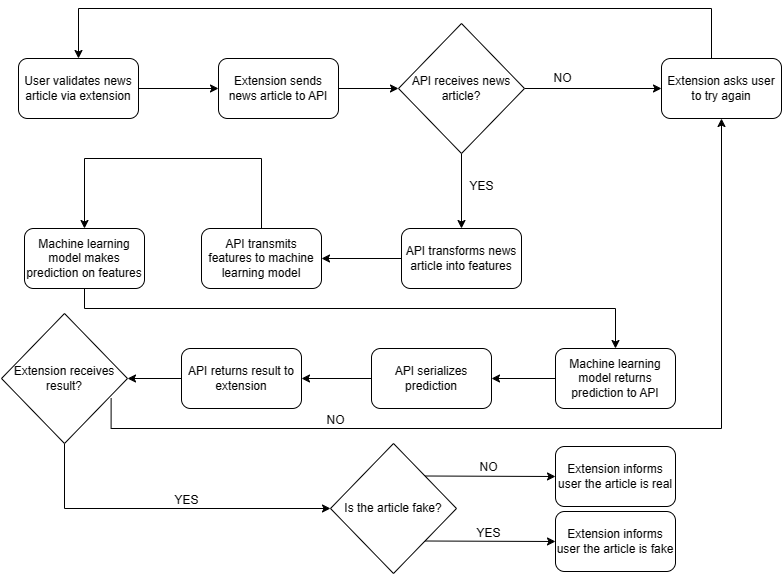
\includegraphics[width=\textwidth,height=\textheight,keepaspectratio]{figures/FakeSystemFlowchart.png}
  \caption{FaKe High Level System Flowchart}
  \label{SystemFlowchart}
\end{figure}
\clearpage

\subsection{System Limitations} \label{extension-limitations}

The FaKe API was hosted on a cloud server that spun down after long periods of inactivity. Free deployment instances at Render spun down after 15 minutes of no inbound traffic \cite{render-docs}, requiring time to spin back up. This meant that it took longer to respond to requests if no request were sent for a long time. Once the server was active, requests may be promptly handled. Due to service and infrastructure constraints, models trained with morphological and lexical features, features that required a Java runtime to be extracted, were unable to be deployed over the web.

The FaKe browser extension as a tool only functioned reliably on news articles written in the Filipino language. Results from making predictions on news articles in English or other languages were unreliable at best. However, the FaKe browser extension had no way of limiting its usage to Filipino language news articles. Furthermore, predictions made by the FaKe browser extension may be inaccurate and may not reflect real-world events. Thus, the responsible usage of the FaKe browser extension rested with the user.

In this regard, we advocate for the hybrid approach in detecting fake news, wherein the employment of the FaKe browser extension is accompanied by dutiful and informed fact-checking. We make no claims that FaKe is a singular catch-all solution to detecting Filipino language fake news.               %LaTeX source file for Chapter 3: Methodology
%   Filename    : chapter_4.tex
\chapter{Results and Discussions}

\section{Dataset}
We built a balanced dataset containing a total of 3206 news articles (1603 real new and 1603 fake news) named Fake News Filipino 2024. This dataset was combined with the Fake News Filipino \cite{fake-news-filipino} dataset into a joint corpus. Figures \ref{fig:oov_data} to \ref{fig:sw_data} depicts the average OOV count, average readability index, and average stop words count of the two datasets. Fake News Filipino 2024 had an average OOV count, readability index, and stop words count of 22.2, 19.7, and 74.5 respectively. On the other hand, retaining the order of the variables, Fake News Filipino had 17.6, 20.5, and 77.8 respectively. On average, news articles in Fake News Filipino were more readable and had a lower count of out-of-vocabulary words as well as a higher number of stop words.

\begin{figure}[h!]
    \centering
    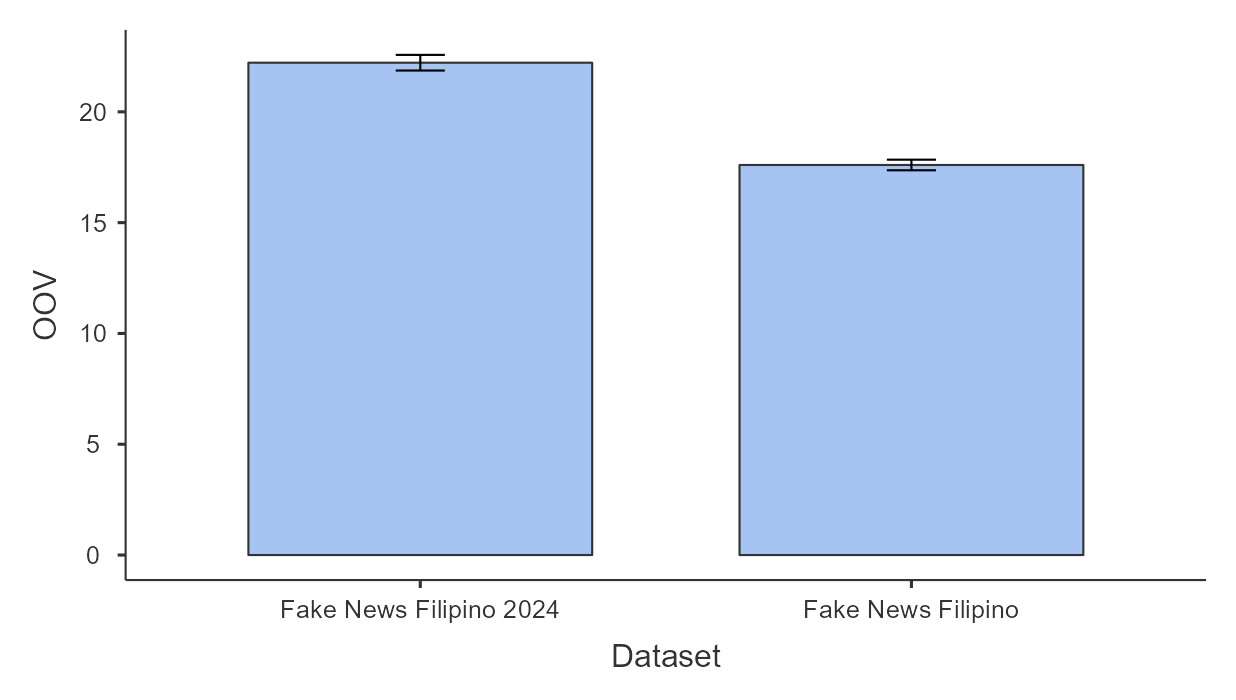
\includegraphics[width=\textwidth,height=\textheight, keepaspectratio]{figures/stats/oov_data.png}
        \caption{Bar plot of average OOV word count of Fake News Filipino and Fake News Filipino 2024.}
        \label{fig:oov_data}
\end{figure}
\begin{figure}[h!]
    \centering
    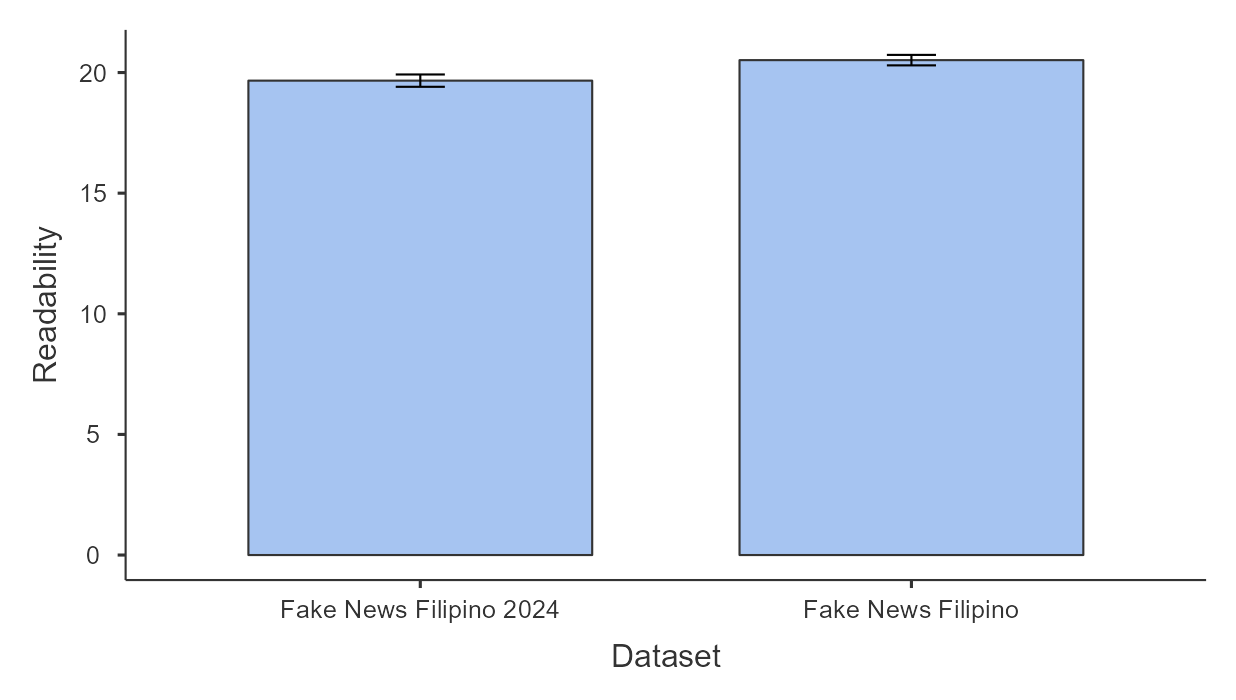
\includegraphics[width=\textwidth,height=\textheight, keepaspectratio]{figures/stats/read_data.png}
        \caption{Bar plot of average readability index of Fake News Filipino and Fake News Filipino 2024.}
        \label{fig:read_data}
\end{figure}
\begin{figure}[h!]
    \centering
    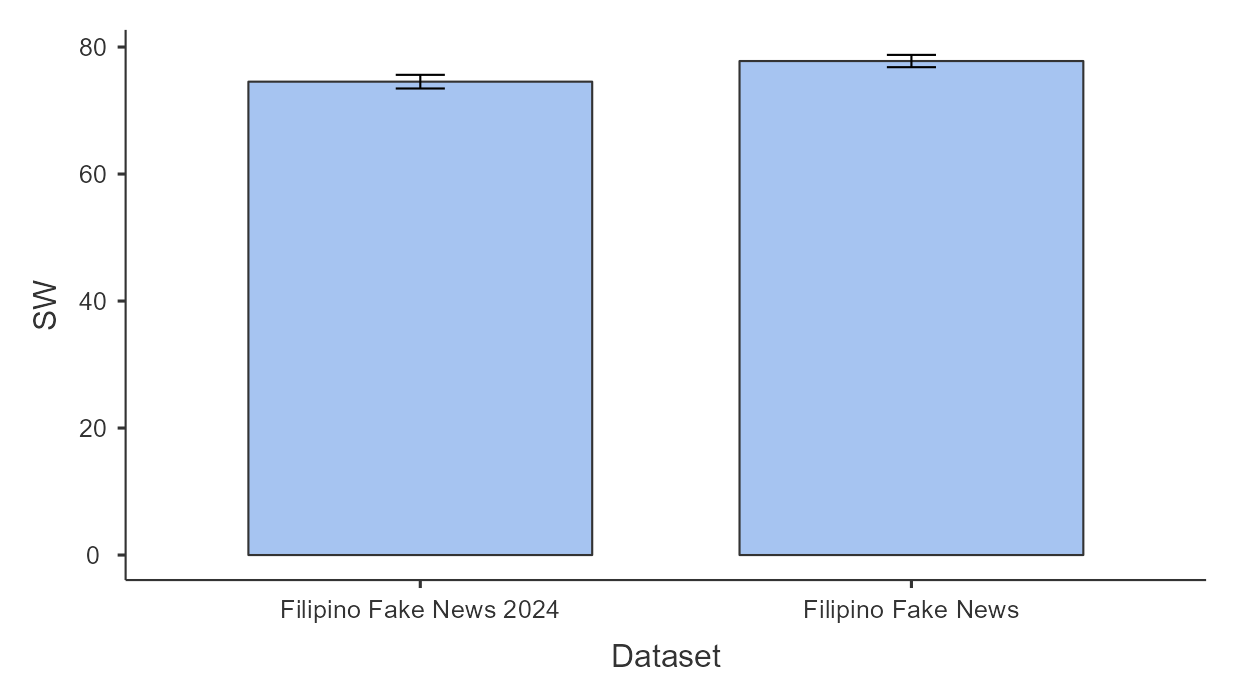
\includegraphics[width=\textwidth,height=\textheight, keepaspectratio]{figures/stats/sw_data.png}
        \caption{Bar plot of average stop word count Fake News Filipino and Fake News Filipino 2024.}
        \label{fig:sw_data}
\end{figure}

\section{Classifiers without Hyperparameter Tuning}

The models were trained on the combined dataset without hyperparameter tuning.

Figure \ref{MNB_default} shows the confusion matrix of \textbf{Multinomial Naive Bayes} without grid search. The model did not misclassify any instance of real news as fake news. However, it misclassified 537 instances of fake news as real news, significantly lowering its recall for fake news. It yielded an accuracy of approximately 0.58. It had the lowest recall for fake news at 0.16, signifying difficulty in identify true instances of fake news and a high false positive rate. The F1-score of real news and fake news were 0.70 and 0.28 respectively. These were relatively low scores.

\begin{figure}[h!]
    \centering
    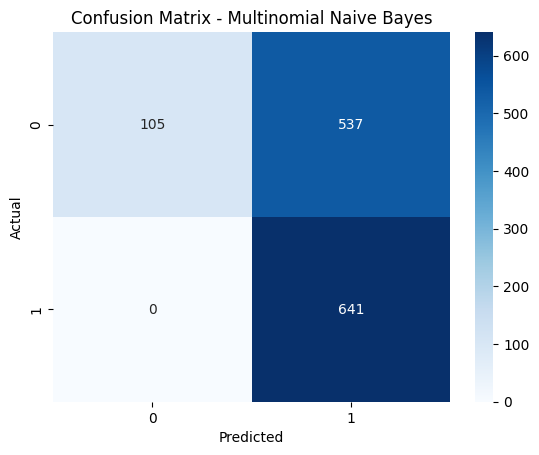
\includegraphics[width=0.6\textwidth,height=0.6\textheight, keepaspectratio]{figures/hyperparam/MNB_default.png}
        \caption{Confusion Matrix of Multinomial Naive Bayes without Grid Search.}
        \label{MNB_default}
\end{figure}

As shown in the confusion matrix of \textbf{Logistic Regression} at Figure \ref{LR_default}, the model misclassified 42 instances of fake news as real news and 51 instances of real news as fake news. It yielded an accuracy of approximately 0.93. It had a high recall for real news and fake news at both 0.93 and 0.92 respectively. The F1-scores for both real news and fake news were 0.93.

\begin{figure}[h!]
    \centering
    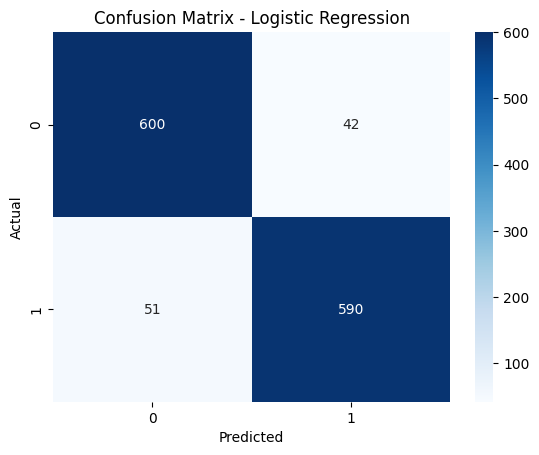
\includegraphics[width=0.6\textwidth,height=0.6\textheight, keepaspectratio]{figures/hyperparam/LR_default.png}
        \caption{Confusion Matrix of Logistic Regression without Grid Search.}
        \label{LR_default}
\end{figure}

Figure \ref{RF_default} depicts the confusion matrix of \textbf{Random Forest}. The model misclassified 66 instances of fake news and 59 instances of real news. It yielded an accuracy of approximately 0.90. It had a recall of 0.90 and 0.91 for fake news and real news respectively. The F1-score of both classes was 0.90, implying balanced metrics.

\begin{figure}[h!]
    \centering
    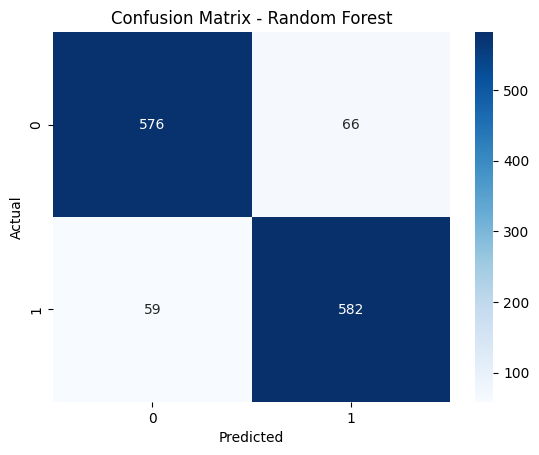
\includegraphics[width=0.6\textwidth,height=0.6\textheight, keepaspectratio]{figures/hyperparam/RF_default.png}
        \caption{Confusion Matrix of Multinomial Naive Bayes without Grid Search.}
        \label{RF_default}
\end{figure}

Based on Figure \ref{SVC_default}, \textbf{Support Vector Classifier}, misclassified 169 instances of fake news and 70 instances of real news. It had an accuracy of approximately 0.81. It had a relatively lower recall for fake news at 0.74. The F1-scores for real news and fake news were 0.80 and 0.83 respectively.

\begin{figure}[h!]
    \centering
    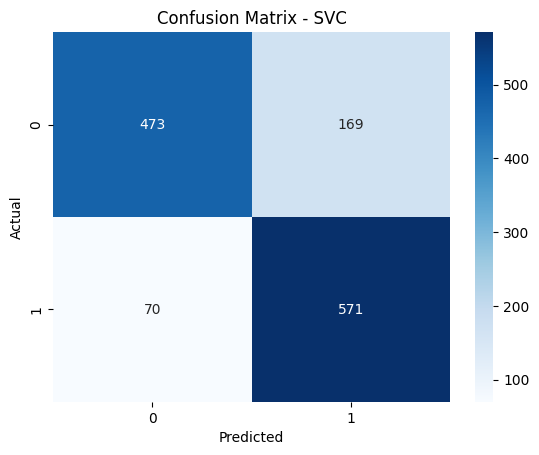
\includegraphics[width=0.6\textwidth,height=0.6\textheight, keepaspectratio]{figures/hyperparam/SVC_default.png}
        \caption{Confusion Matrix of Multinomial Naive Bayes without Grid Search.}
        \label{SVC_default}
\end{figure}

Results without hyperparameter tuning are summarized in Table \ref{tab:no_hyperparam_summary}. As shown in Table \ref{tab:no_hyperparam_summary}, Logistic Regression had the highest F1-scores while Multinomial Naive Bayes scored the lowest.

\begin{table}[ht]
    \centering
    \begin{tabular}{|l|ccc|ccc|}
    \hline
    & \multicolumn{3}{c|}{Multinomial Naive Bayes} & \multicolumn{3}{c|}{Logistic Regression} \\
    \hline
    & Precision & Recall & F1-score & Precision & Recall & F1-score \\
    \hline
    Fake & 1.00 & 0.16 & 0.28 & 0.92 & 0.93 & 0.93 \\
    Not Fake & 0.54 & 1.00 & 0.70 & 0.93 & 0.92 & 0.93 \\
    Accuracy & & & 0.58 & & & 0.93 \\
    \hline
    & \multicolumn{3}{c|}{Random Forest} & \multicolumn{3}{c|}{Support Vector Classifier} \\
    \hline
    & Precision & Recall & F1-score & Precision & Recall & F1-score \\
    \hline
    Fake & 0.91 & 0.90 & 0.90 & 0.87 & 0.74 & 0.80 \\
    Not Fake & 0.90 & 0.91 & 0.90 & 0.77 & 0.89 & 0.83 \\
    Accuracy & & & 0.90 & & & 0.81 \\
    \hline
    \end{tabular}
    \caption{Performance metrics for classifiers without hyperparameter tuning.}
    \label{tab:no_hyperparam_summary}
\end{table}



\section{Classifiers with Hyperparameter Tuning}
\label{sec:ParamTuning}
To the determine the optimal hyperparameters, all models were trained and tested on the combined dataset using grid search with five-fold cross validation.

Figure \ref{MNB_hyperparam} shows the performance of \textbf{Multinomial Naive Bayes} with an alpha of 0.01, the optimal hyperparameter based on the cross validation. The model misclassified 155 instances of fake news and 18 instances of real news. It yielded an accuracy of approximately 0.865. It had the lowest recall for fake news at 0.87.

\begin{figure}[h!]
\centering
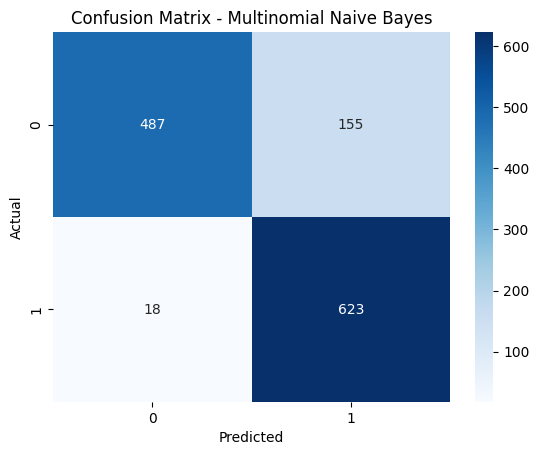
\includegraphics[width=0.6\textwidth,height=0.6\textheight, keepaspectratio]{figures/hyperparam/MNB.png}
    \caption{Confusion Matrix of Multinomial Naive Bayes with alpha = 0.01.}
    \label{MNB_hyperparam}
\end{figure}

The best hyperparameter for \textbf{Logistic Regression} was max\_iter = 2000. As shown in Figure \ref{LR_hyperparam}, Logistic Regression misclassified 42 instances of fake news and 51 instances of real news. It yielded an accuracy of 0.928 and an F1-score of 0.93 for both real news and fake news.

\begin{figure}[h!]
\centering
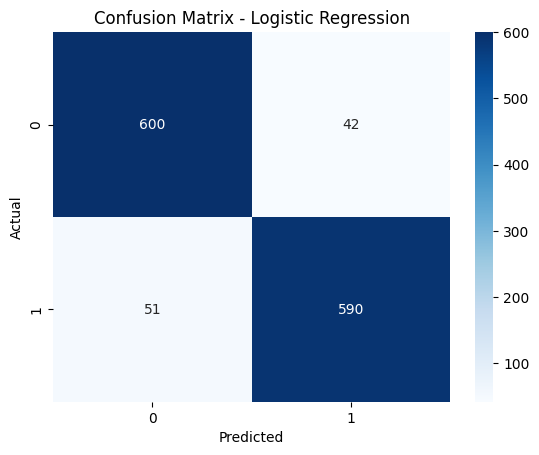
\includegraphics[width=0.6\textwidth,height=0.6\textheight, keepaspectratio]{figures/hyperparam/LR.png}
    \caption{Confusion Matrix of Linear Regression with max\_iter = 2000.}
    \label{LR_hyperparam}
\end{figure}

For \textbf{Random Forest}, max\_depth = 20 was the optimal hyperparameter. The performance of Random Forest is shown in Figure \ref{RF_hyperparam}. The model misclassified 80 instances of fake news and 63 instances of real news. It yielded an accuracy of 0.889 with an F1-score of 0.89 for both fake news and real news.

\begin{figure}[h!]
\centering
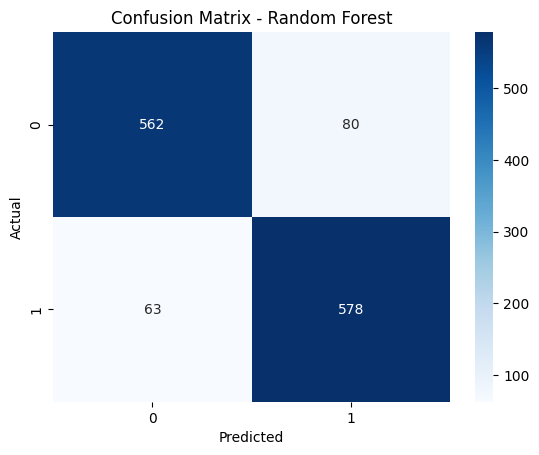
\includegraphics[width=0.6\textwidth,height=0.6\textheight, keepaspectratio]{figures/hyperparam/RF.png}
    \caption{Confusion Matrix of Random Forest with max\_depth = 20.}
    \label{RF_hyperparam}
\end{figure}

For \textbf{Support Vector Classifier}, the optimal hyperparameter was C = 0.1 with a linear kernel. As shown in Figure \ref{SVC_hyperparam}, the model misclassified 42 instances of fake news and 51 instances of real news. It yielded an accuracy of 0.928 and an F1-score of 0.93 for both fake news and real news.

Both Support Vector Classifier and Logistic Regression yielded the highest accuracy with hyperparameter tuning.

\begin{figure}[h!]
\centering
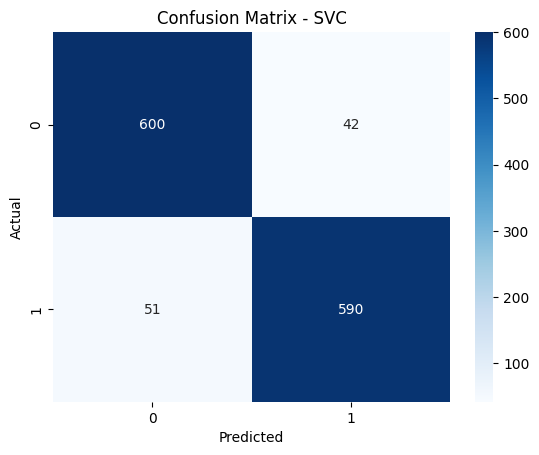
\includegraphics[width=0.6\textwidth,height=0.6\textheight, keepaspectratio]{figures/hyperparam/SVC.png}
    \caption{Confusion Support Vector Classifier with a linear kernel and C = 0.1.}
    \label{SVC_hyperparam}
\end{figure}

The results are summarized in Table \ref{tab:hyperparam_summary}. Both Logistic Regression and Support Vector Classifier scored the highest F1-scores while Random Forest scored the lowest. Comparing the accuracies of the classifiers without hyperparameter tuning in Table \ref{tab:no_hyperparam_summary} and their accuracies with hyperparameter tuning in Table \ref{tab:hyperparam_summary}, hyperparameter tuning significantly increased the accuracy of Multinomial Naive Bayes and Support Vector Classifier. However, hyperparameter tuning did not have any significant impact on the accuracies of Logistic Regression and Random Forest.

\begin{table}[ht]
    \centering
    \begin{tabular}{|l|ccc|ccc|}
    \hline
    & \multicolumn{3}{c|}{Multinomial Naive Bayes} & \multicolumn{3}{c|}{Logistic Regression} \\
    \hline
    & Precision & Recall & F1-score & Precision & Recall & F1-score \\
    \hline
    Fake & 0.93 & 0.76 & 0.85 & 0.92 & 0.93 & 0.93 \\
    Not Fake & 0.80 & 0.97 & 0.88 & 0.93 & 0.92 & 0.93 \\
    Accuracy & & & 0.87 & & & 0.93 \\
    \hline
    & \multicolumn{3}{c|}{Random Forest} & \multicolumn{3}{c|}{Support Vector Classifier} \\
    \hline
    & Precision & Recall & F1-score & Precision & Recall & F1-score \\
    \hline
    Fake & 0.90 & 0.88 & 0.89 & 0.92 & 0.93 & 0.93 \\
    Not Fake & 0.88 & 0.90 & 0.89 & 0.93 & 0.92 & 0.93 \\
    Accuracy & & & 0.89 & & & 0.93 \\
    \hline
    \end{tabular}
    \caption{Performance metrics for classifiers with hyperparameter tuning.}
    \label{tab:hyperparam_summary}
\end{table}

\section{Accuracy Testing}

Using the optimal hyperparameters in Section \ref{sec:ParamTuning}, all four models were trained and tested using five-fold cross validation six times, a total of 30 tests, across three datasets: Fake News Filipino (2020), Fake News Filipino 2024 (2024), and the combined corpus with the two datasets. Average accuracies of the models are shown in Table \ref{tab::AverageAccuracies}. Logistic Regression and Support Vector Classifier scored the highest average accuracy in both Fake News Filipino and Fake News Filipino 2024. But for the combined dataset, only Logistic Regression yielded the highest average accuracy. Compared to the other models across the three datasets, Multinomial Naive Bayes and Random Forest performed relatively worst in the combined dataset with accuracies of 86.0\% and 88.8\% respectively. Table \ref{tab::AverageAccuracies} shows the average accuracies of the models. The box plot of the accuracies is depicted in Figure \ref{fig:box_plot_accuracy}.

\begin{tabularx}{\textwidth}{|l|l|c|}
    \hline Classifier & Dataset & Average Accuracy \\ \hline
    \endfirsthead

    \hline
    \multicolumn{3}{|r|}
    {Continued from previous page.} \\
    \hline
    Classifier & Dataset & Average Accuracy \\ \hline
    \endhead

    \hline \multicolumn{3}{|r|}{{Continued on next page...}} \\ \hline
    \endfoot

    \hline
    \caption{Average Accuracies of classifiers for each dataset.}
    \endlastfoot

    Logistic Regression & Fake News Filipino & 0.951 \\
    & Fake News Filipino 2024 & 0.947\\
    & Combined & 0.924 \\
    \hline
    Multinomial Naive Bayes & Fake News Filipino & 0.923 \\
    & Fake News Filipino 2024 & 0.885 \\
    & Combined & 0.860 \\
    \hline
    Random Forest & Fake News Filipino & 0.919 \\
    & Fake News Filipino 2024 & 0.926 \\
    & Combined & 0.888 \\
    \hline
    Support Vector Classifier & Fake News Filipino & 0.951 \\
    & Fake News Filipino 2024 & 0.947 \\
    & Combined & 0.922
\label{tab::AverageAccuracies}
\end{tabularx}

\begin{figure}[h!]
    \centering
    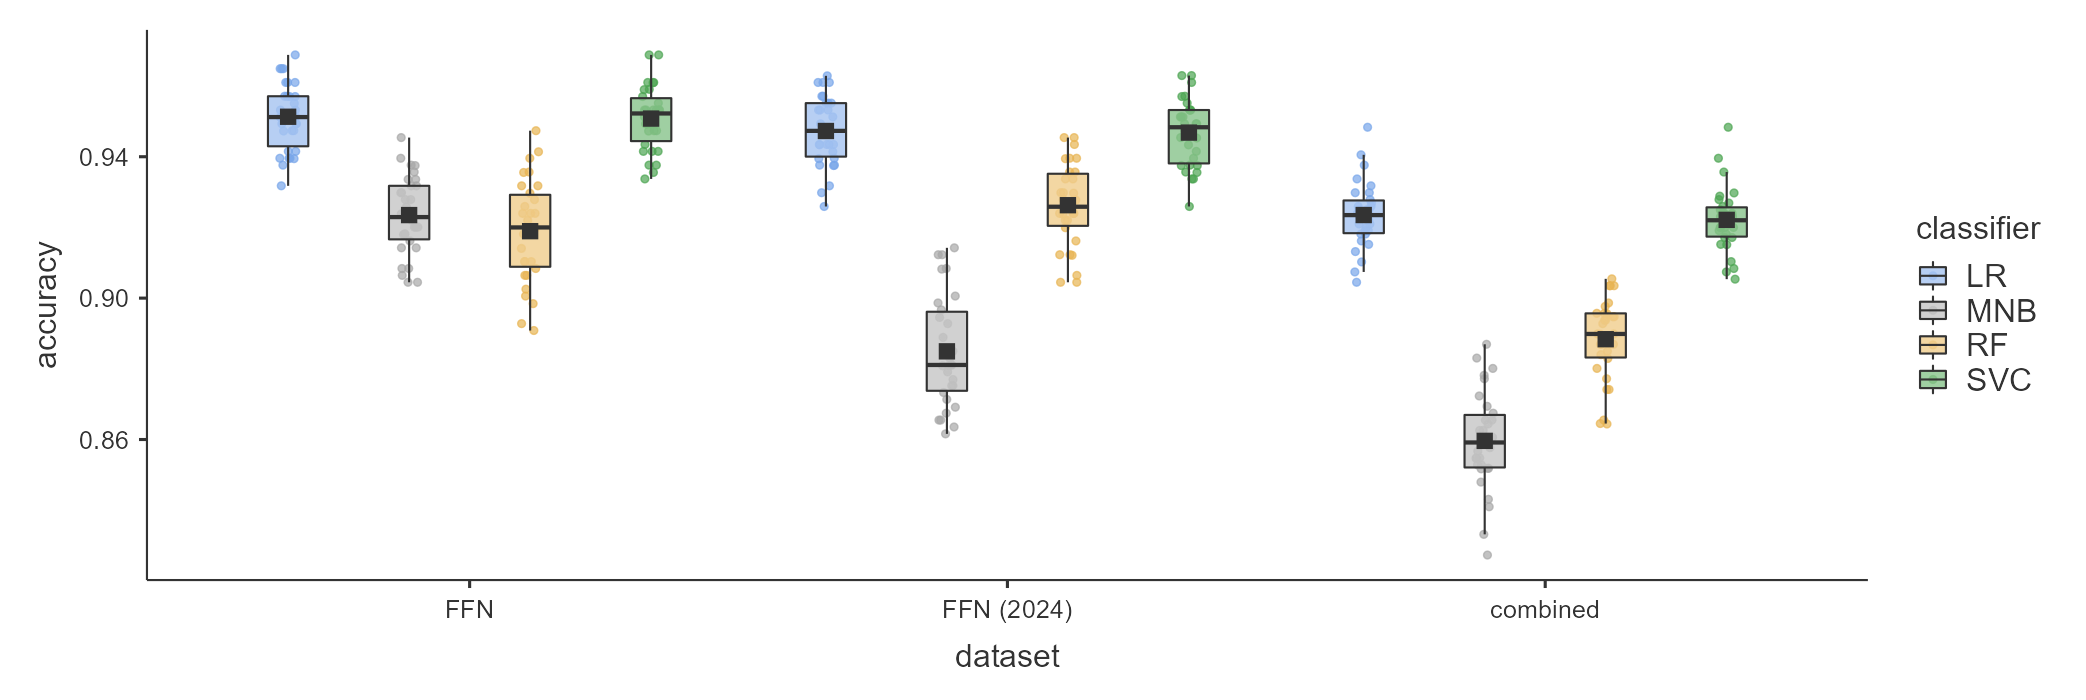
\includegraphics[width=\textwidth,height=\textheight, keepaspectratio]{figures/stats/box_plot.png}
        \caption{Box plot of the accuracies accross datasets.}
        \label{fig:box_plot_accuracy}
\end{figure}

The Shapiro-Wilk test was used to assess the normality of each group in a two-way format, where accuracies were the dependent variable, and datasets and classifiers were the factors. As shown in Table \ref{tab::normality_tests}, all groups have \textit{p}-values greater than or equal to 0.05 indicating that the data is normally distributed in the two-way format. However, with a \textit{p}-value (0.003) lower than 0.05, Levene's test determined the variances of the groups to be heterogenous.

\pagebreak

\begin{tabularx}{\textwidth}{|l|l|l|l|}
    \hline
    Dataset & Classifier & Statistic & \textit{p}-value \\
    \hline
    Fake News Filipino & LR & 0.968 & 0.492 \\
    & MNB & 0.971 & 0.571 \\
    & RF & 0.985 & 0.938 \\
    & SVC & 0.972 & 0.603 \\
    \hline
    Fake News Filipino 2024 & LR & 0.963 & 0.363 \\
    & MNB & 0.940 & 0.928 \\
    & RF & 0.962 & 0.342 \\
    & SVC & 0.972 & 0.598 \\
    \hline
    Combined & LR & 0.979 & 0.793 \\
    & MNB & 0.981 & 0.852 \\
    & RF & 0.934 & 0.063 \\
    & SVC & 0.950 & 0.164 \\
    \hline
\caption{Shapiro-Wilk normality test in a two-way format.}
\label{tab::normality_tests}
\end{tabularx}

To determine if there were significant differences between accuracies of different classifiers in different datasets, and taking into account the heteroscedacity of the data, two-way ANOVA for trimmed means was performed. As shown in Table \ref{tab::two-way} there was a significant difference (\textit{p}-value = 0.001) between accuracies in different datasets averaged across the classifiers. Additionally, there was a significant difference (\textit{p}-value = 0.001) between accuracies in the classifiers averaged across the datasets. Furthermore, their interaction effect was also significant (\textit{p}-value = 0.001). Thus, accuracy was affected both by the main effects of the dataset and classifier and also their combinations.

\begin{tabularx}{\textwidth}{|l|l|l|}
    \hline
    Factor & Statistic & \textit{p}-value \\
    \hline
    dataset & 689.45 & 0.001 \\
    \hline
    classifier & 1010.0371 & 0.001 \\
    \hline
    dataset*classifier & 129.07 & 0.001 \\
    \hline
\caption{Two-way ANOVA for Trimmed Means.}
\label{tab::two-way}
\end{tabularx}

To determine which classifiers had significant differences within the different datsets, post-hoc mean-separation testing was conducted using Bonferroni Correction for subgroups of each dataset level. As shown in Table \ref{tab::post-hoc-dataset-lvl}, the only subgroups that did not have significant differences were Logistic Regression and Support Vector Classifier across all datasets, as well as Multinomial Naive Bayes and Random Forest in the Fake News Filipino dataset.

The results were reflected in the interaction plot of the accuracies in Figure \ref{fig:interaction_plot}. As shown in Figure \ref{fig:interaction_plot}, the accuracies of Logistic Regression and Support Vector Classifier were almost equal across all datasets. The same could be said for the accuracy of Multinomial Naive Bayes and Random Forest in the Fake News Filipino dataset. It could also be observed that the performance of the classifiers changes depending on the dataset just as the two-way ANOVA suggested.

To determine which classifiers had significant differences between datasets, a similar post-hoc test was conducted for subgroups of each classifier level. Table \ref{tab::post-hoc-classifier-lvl} shows that only Multinomial Naive Bayes had a significant change in performance between Fake News Filipino 2024 and Fake News Filipino dataset. Furthermore, all accuracies of the classifiers differ significantly in the combined dataset compared with their accuracies in either Fake News Filipino or Fake News Filipino 2024.

\begin{figure}[h!]
    \centering
    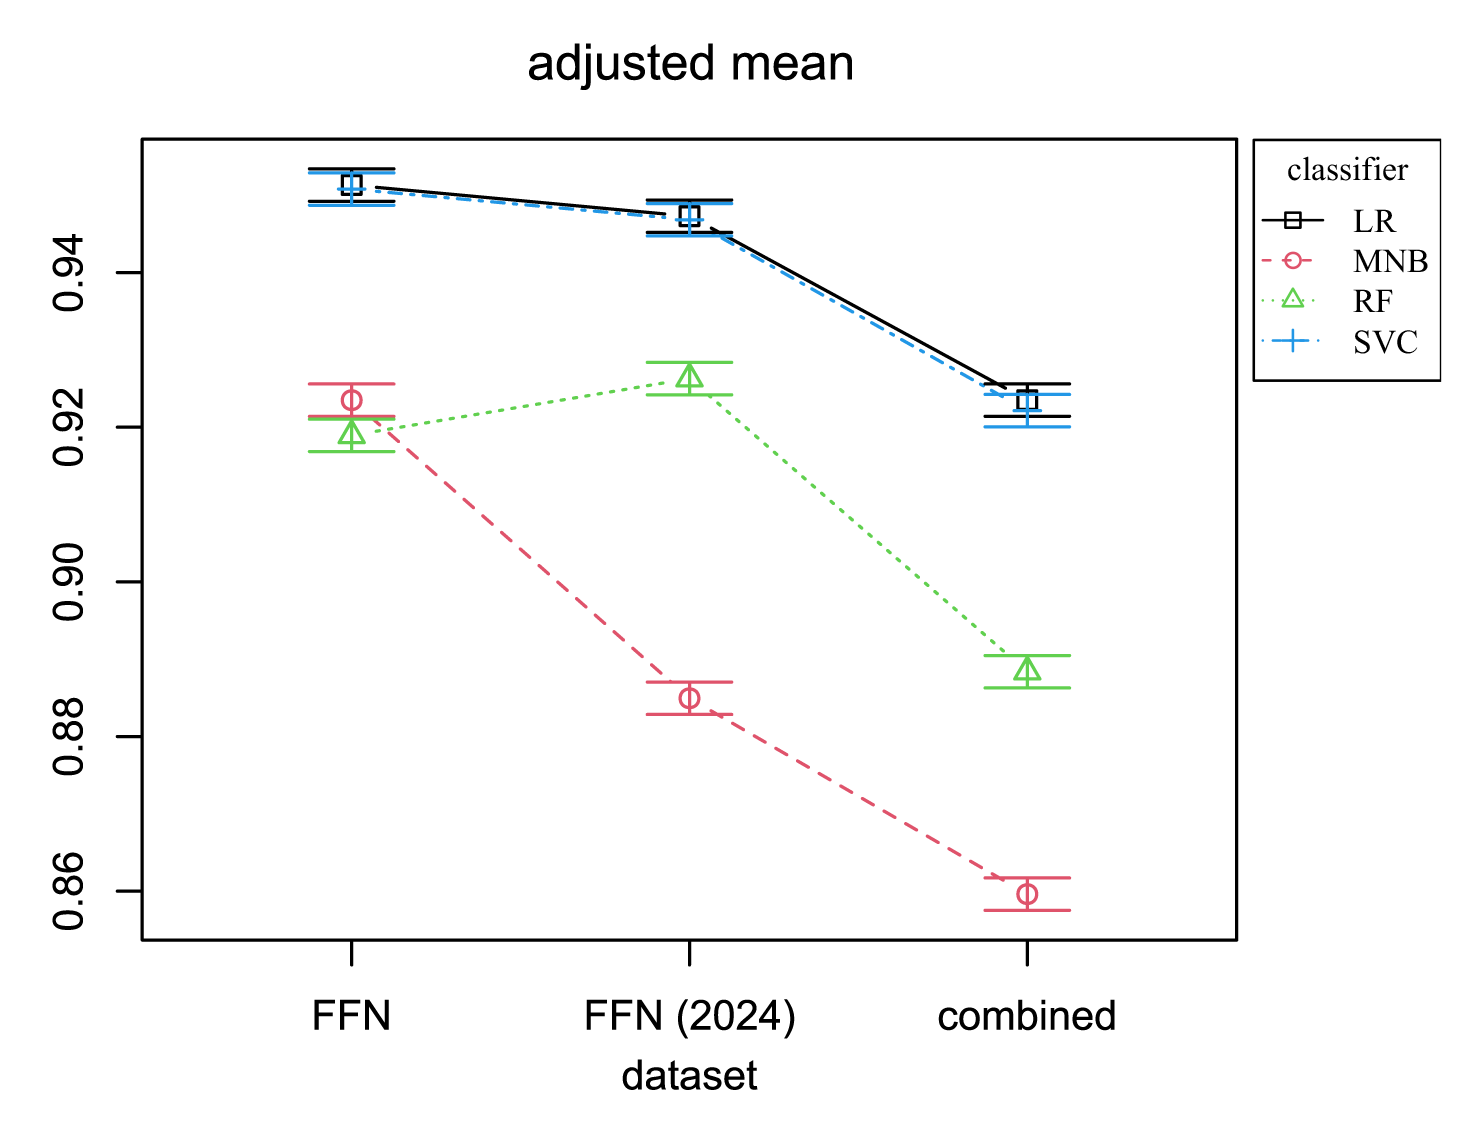
\includegraphics[width=\textwidth,height=\textheight, keepaspectratio]{figures/stats/im.png}
        \caption{Interaction plot of accuracies across datasets.}
        \label{fig:interaction_plot}
\end{figure}

\begin{tabularx}{\textwidth}{|l|l|l|l|}
    \hline Dataset & Classifier (a) & Classifier(b) & \textit{p}-value \\ \hline
    \endfirsthead

    \hline
    \multicolumn{4}{|r|}
    {Continued from previous page.} \\

    \hline
    Dataset & Classifier (a) & Classifier(b) & \textit{p}-value \\ \hline
    \endhead

    \hline \multicolumn{4}{|r|}{{Continued on next page...}} \\ \hline
    \endfoot

    \hline
    \caption{Bonferroni correction for subgroups of each dataset level.}
    \endlastfoot

    Fake News Filipino & LR & MNB & \textless 0.001 \\
    \cline{3-4}
    & & RF & \textless 0.001 \\
    \cline{3-4}
    & & SVC & 1.00 \\
    \cline{2-4}
    & MNB & RF & 1.00 \\
    \cline{3-4}
    & & SVC & \textless 0.001 \\
    \cline{2-4}
    & RF & SVC & \textless 0.001 \\
    \hline
    Fake News Filipino 2024 & LR & MNB & \textless 0.001 \\
    \cline{3-4}
    & & RF & \textless 0.001 \\
    \cline{3-4}
    & & SVC & 1.00 \\
    \cline{2-4}
    & MNB & RF & \textless 0.001 \\
    \cline{3-4}
    & & SVC & \textless 0.001 \\
    \cline{2-4}
    & RF & SVC & \textless 0.001 \\
    \hline
    Combined & LR & MNB & \textless 0.001 \\
    \cline{3-4}
    & & RF & \textless 0.001 \\
    \cline{3-4}
    & & SVC & 1.00 \\
    \cline{2-4}
    & MNB & RF & \textless 0.001 \\
    \cline{3-4}
    & & SVC & \textless 0.001 \\
    \cline{2-4}
    & RF & SVC & \textless 0.001
\label{tab::post-hoc-dataset-lvl}
\end{tabularx}

\begin{tabularx}{\textwidth}{|l|l|l|l|}
    \hline Classifier & Dataset(a) & Dataset(b) & \textit{p}-value \\ \hline
    \endfirsthead

    \hline
    \multicolumn{4}{|r|}
    {Continued from previous page.} \\

    \hline
    Classifier & Dataset(a) & Dataset(b) & \textit{p}-value \\ \hline
    \endhead

    \hline \multicolumn{4}{|r|}{{Continued on next page...}} \\ \hline
    \endfoot

    \hline
    \caption{Bonferroni correction for subgroups of each classifier level.}
    \endlastfoot

    LR & Fake News Filipino & Fake News Filipino 2024 & 0.485 \\
    \cline{3-4}
    & & Combined & \textless 0.001 \\
    \cline{2-4}
    & Fake News Filipino 2024 & Combined & \textless 0.001 \\
    \hline
    MNB & Fake News Filipino & Fake News Filipino 2024 & \textless 0.001 \\
    \cline{3-4}
    & & Combined & \textless 0.001 \\
    \cline{2-4}
    & Fake News Filipino 2024 & Combined & \textless 0.001 \\
    \hline
    RF & Fake News Filipino & Fake News Filipino 2024 & 0.150 \\
    \cline{3-4}
    & & Combined & \textless 0.001 \\
    \cline{2-4}
    & Fake News Filipino 2024 & Combined & \textless 0.001 \\
    \hline
    SVC & Fake News Filipino & Fake News Filipino 2024 & 0.421 \\
    \cline{3-4}
    & & Combined & \textless 0.001 \\
    \cline{2-4}
    & Fake News Filipino 2024 & Combined & \textless 0.001
\label{tab::post-hoc-classifier-lvl}
\end{tabularx}

\pagebreak
\section{App Testing}
The FaKe application was assessed using three prominent browsers - Google Chrome, Microsoft Edge, and Mozilla Firefox. The evaluation utilized identical articles categorized as fake news or real news. Figure \ref{fig:fake-chrome-test} and \ref{fig:real-chrome-test} illustrate the outcomes using Google Chrome,  Figure \ref{fig:fake-edge-test} and \ref{fig:real-edge-test} display the results for Microsoft Edge, and Figure \ref{fig:fake-firefox-test} and \ref{fig:real-firefox-test} show the findings for Mozilla Firefox. The results demonstrate uniformity of the application's functionality through different browsers.

    \begin{figure}[h!]
        \centering
        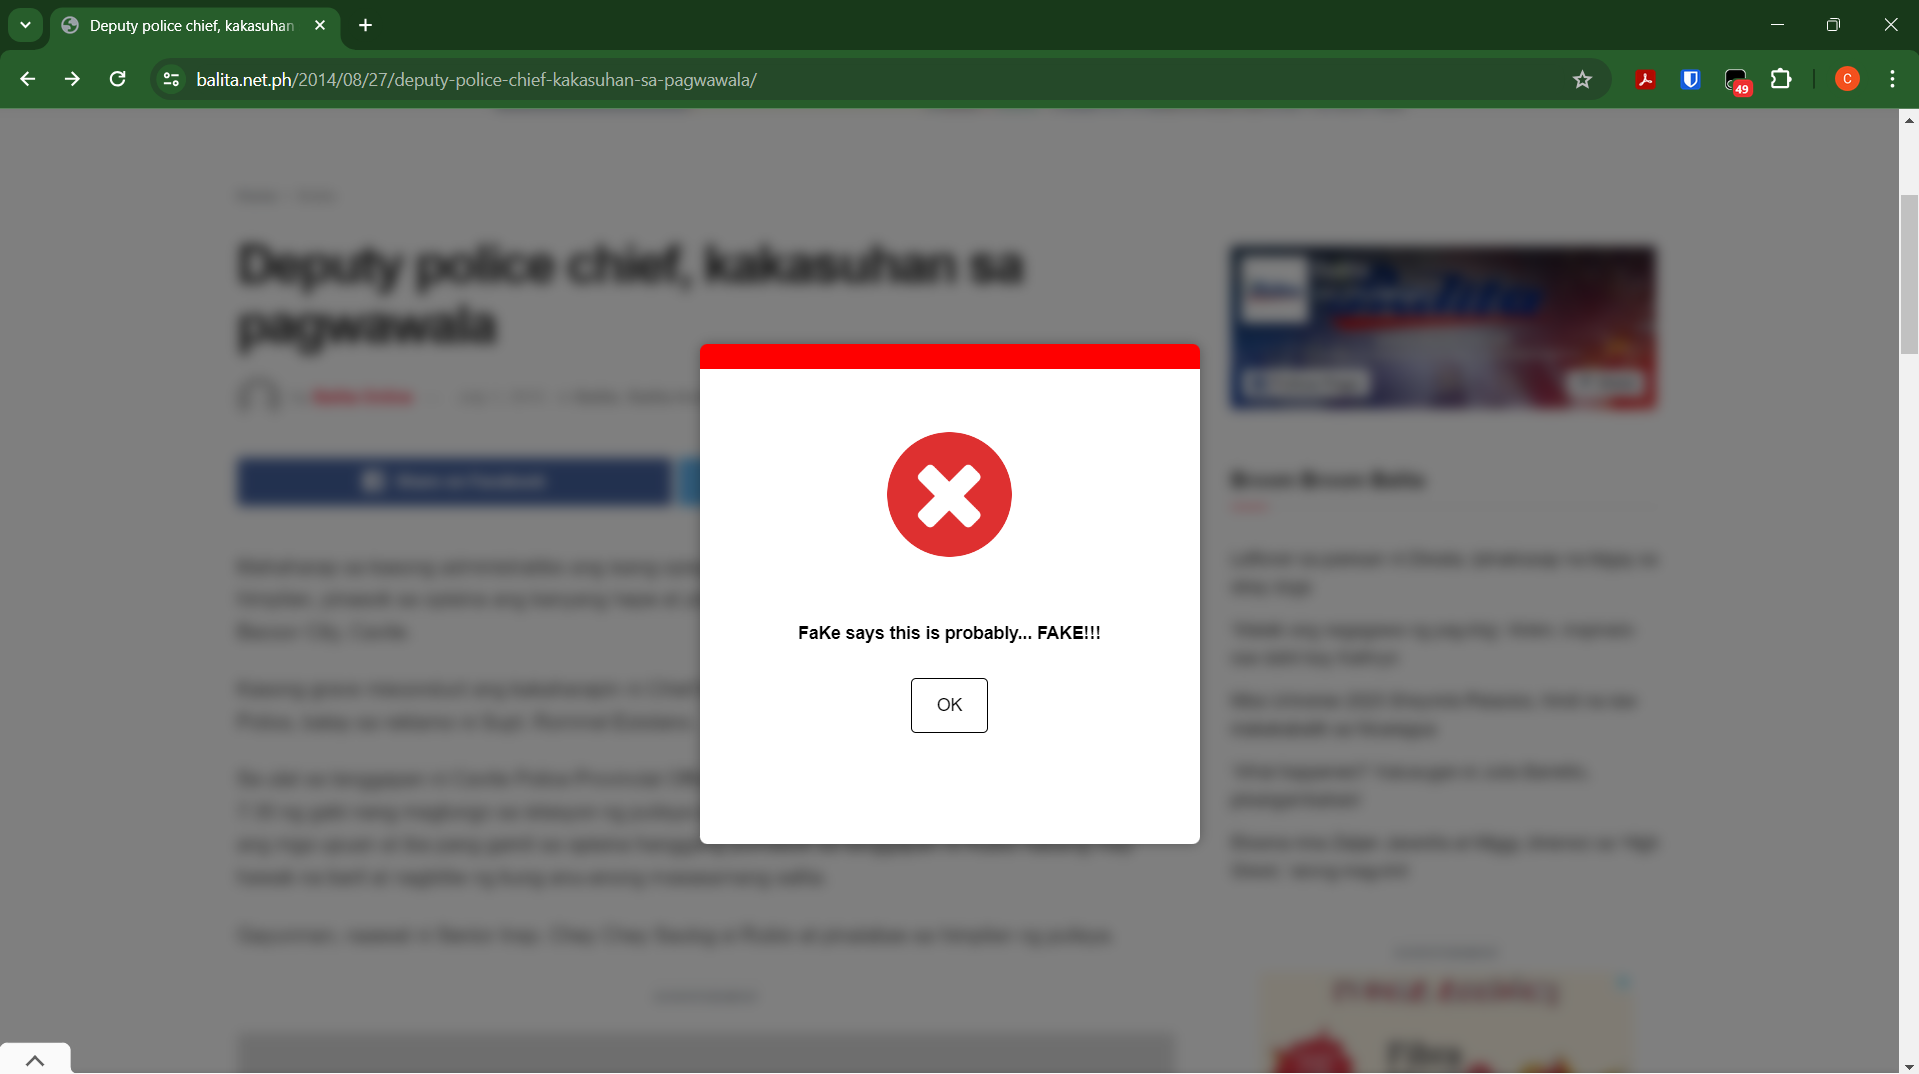
\includegraphics[width=1\textwidth,height=1\textheight, keepaspectratio]{figures/Screenshots/chrome-fake.png}
            \caption{Fake App testing with Google Chrome.}
            \label{fig:fake-chrome-test}
        \end{figure}

        \begin{figure}[h!]
            \centering
            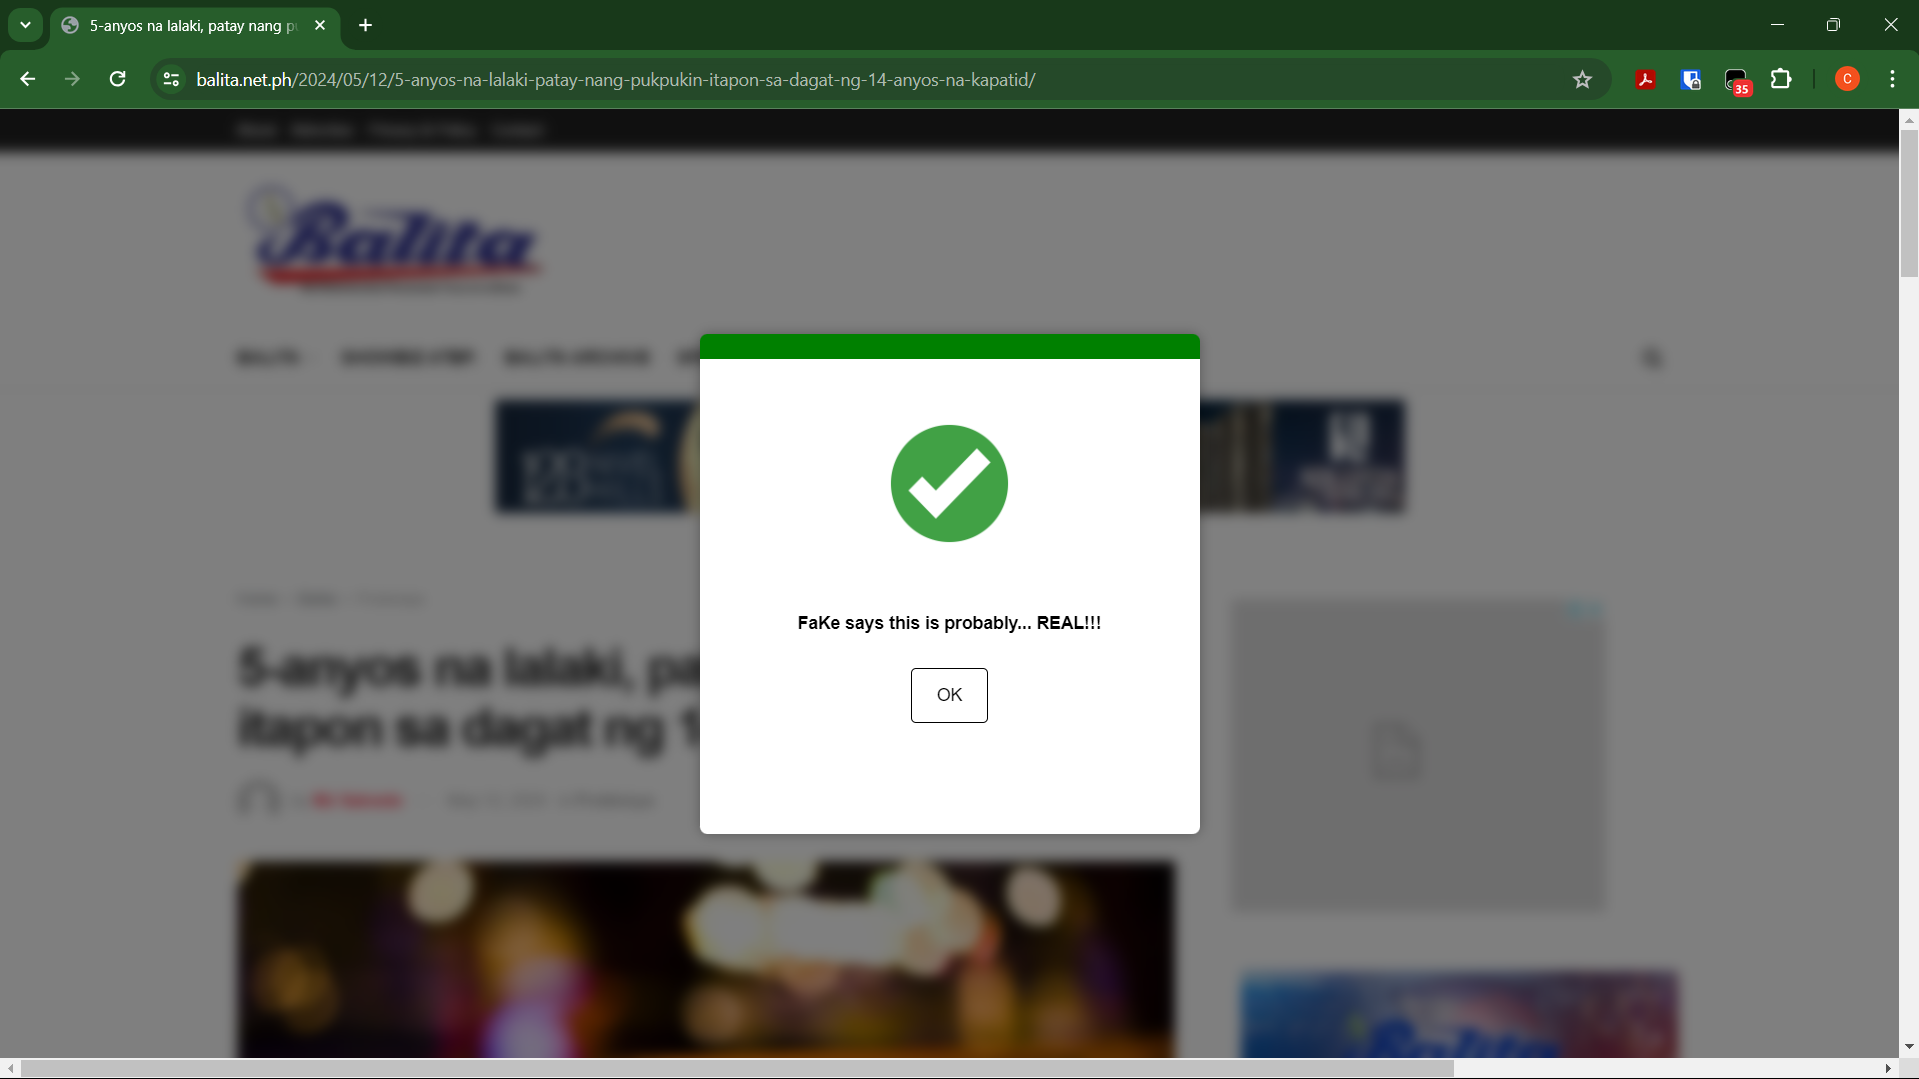
\includegraphics[width=1\textwidth,height=1\textheight, keepaspectratio]{figures/Screenshots/chrome-real.png}
                \caption{Real App testing with Google Chrome.}
                \label{fig:real-chrome-test}
            \end{figure}

            \begin{figure}[h!]
                \centering
                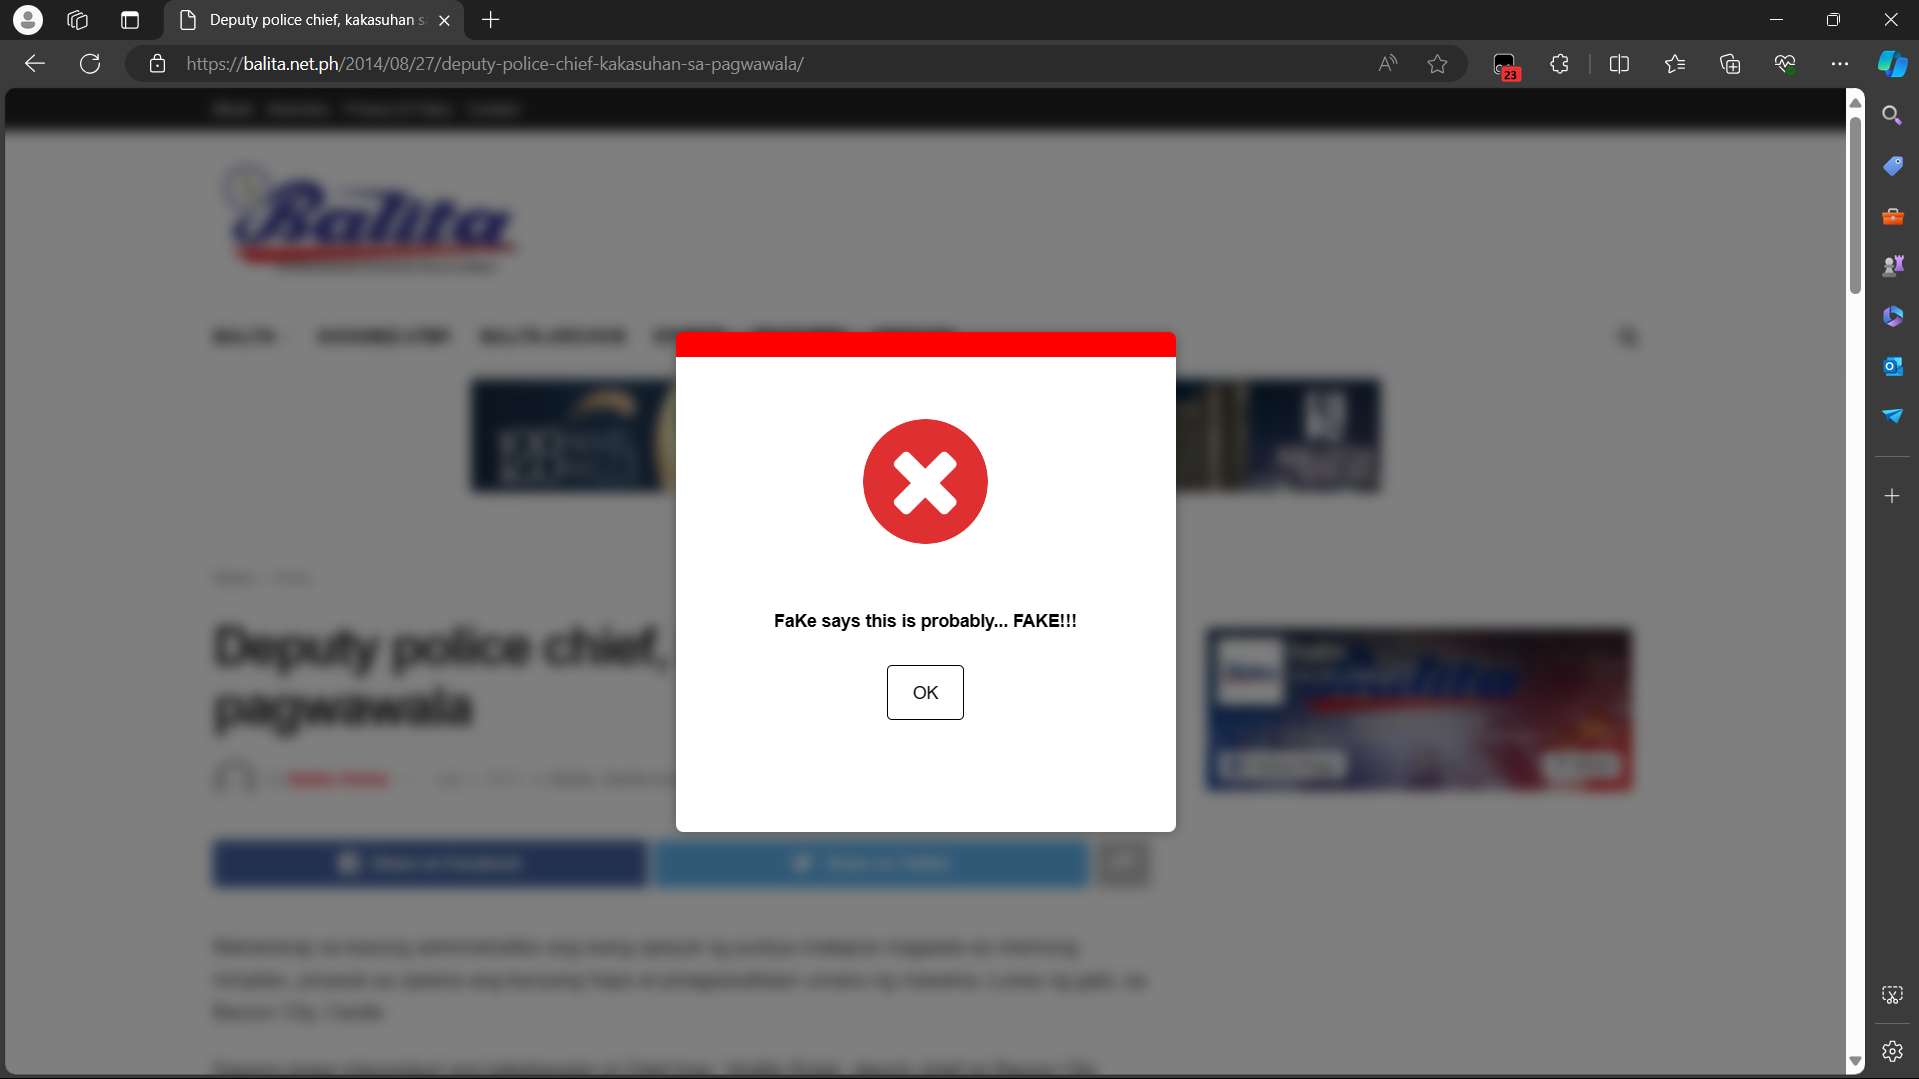
\includegraphics[width=1\textwidth,height=1\textheight, keepaspectratio]{figures/Screenshots/edge-fake.png}
                    \caption{Fake App testing with Microsoft Edge.}
                    \label{fig:fake-edge-test}
                \end{figure}

            \begin{figure}[h!]
                \centering
                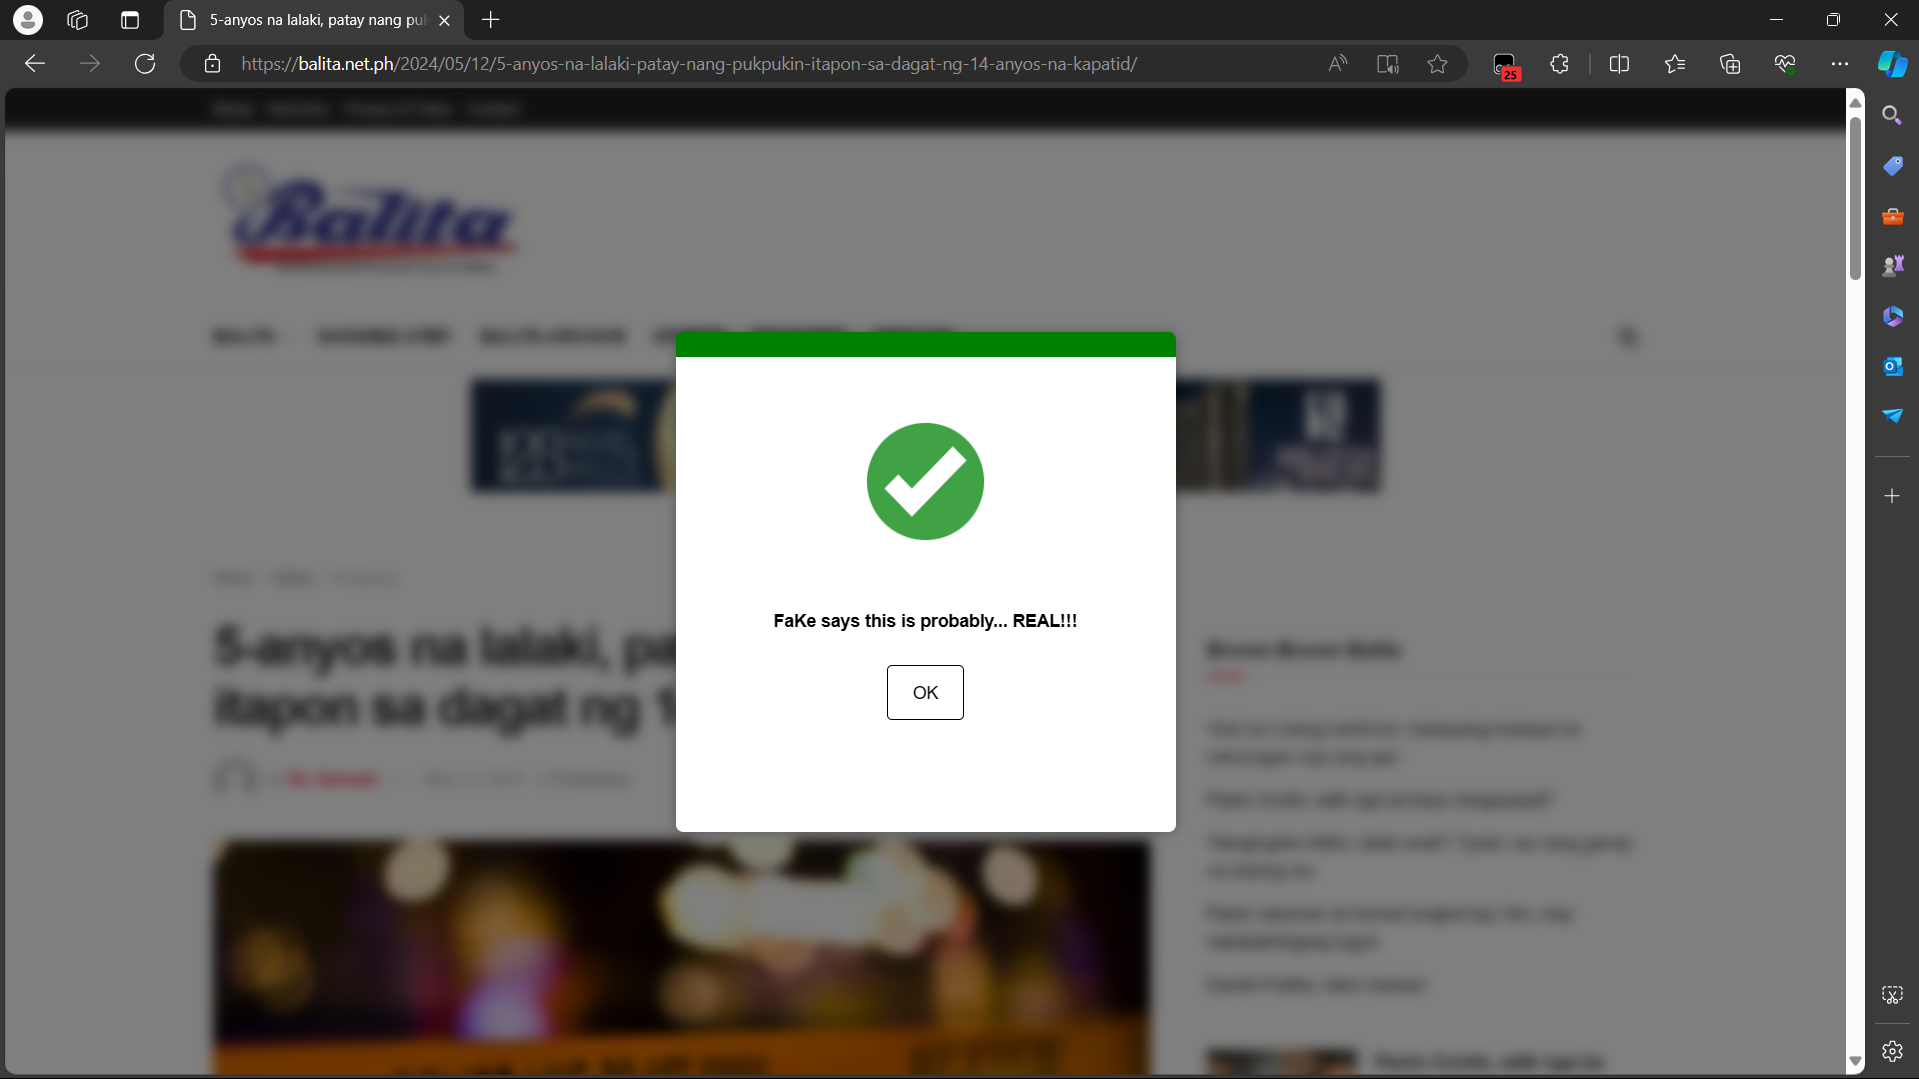
\includegraphics[width=1\textwidth,height=1\textheight, keepaspectratio]{figures/Screenshots/edge-real.png}
                    \caption{Real App testing with Microsoft Edge.}
                    \label{fig:real-edge-test}
                \end{figure}

            \begin{figure}[h!]
                \centering
                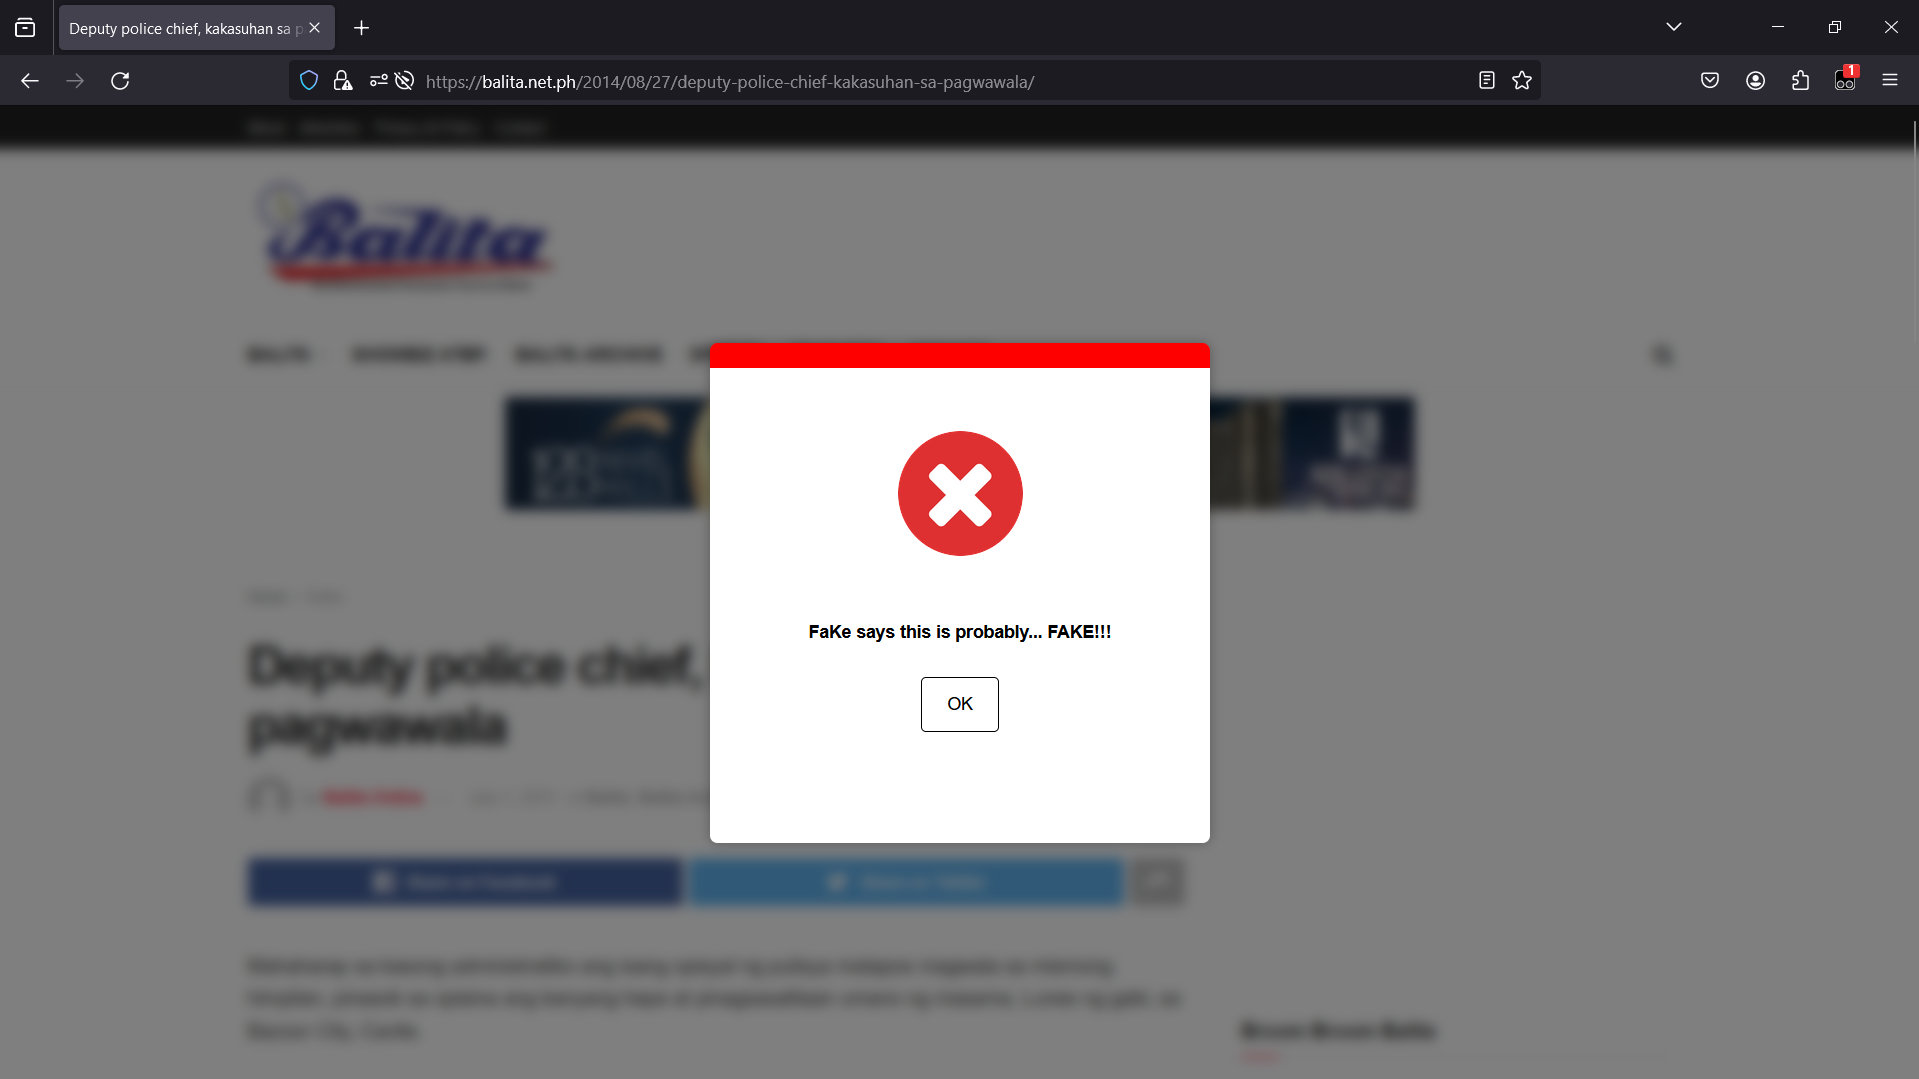
\includegraphics[width=1\textwidth,height=1\textheight, keepaspectratio]{figures/Screenshots/firefox-fake.png}
                    \caption{Fake App testing with Mozilla Firefox.}
                    \label{fig:fake-firefox-test}
                \end{figure}

            \begin{figure}[h!]
                \centering
                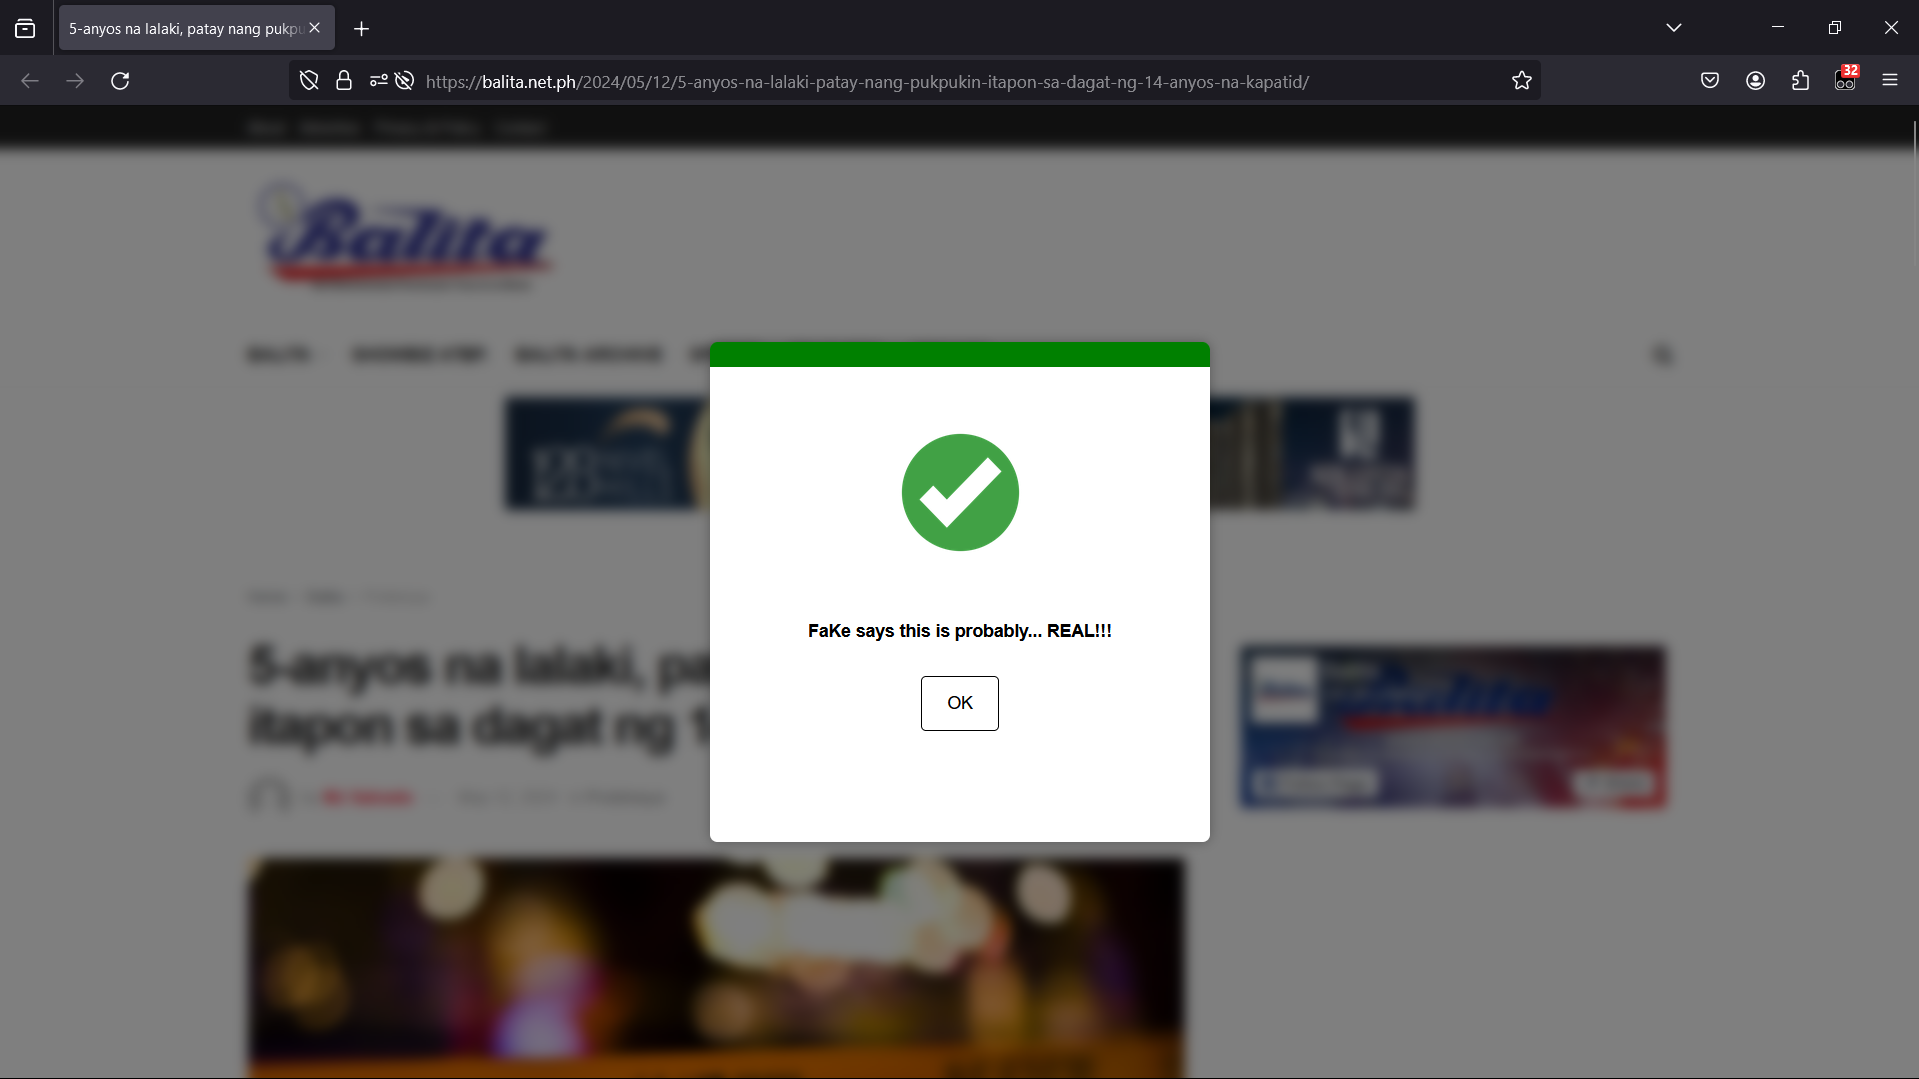
\includegraphics[width=1\textwidth,height=1\textheight, keepaspectratio]{figures/Screenshots/firefox-real.png}
                    \caption{Real App testing with Mozilla Firefox.}
                    \label{fig:real-firefox-test}
                \end{figure}
\clearpage
\pagebreak
\section{Summary} \label{dataset-limitation}

As shown in the results of two-way ANOVA together with the post-hoc tests, three out of four classifiers, namely Logistic Regression, Random Forest, and Support Vector Classifier, did not exhibit a significant change in performance between Fake News Filipino and Fake News Filipino 2024. However, the accuracies of all classifiers were significantly lower on the joint corpus. The reason for this may be attributed to differences in the writing styles of the news articles found between the two datasets. This hypothesis is supported by the differences in the number of out-of-vocabulary words, the average number of stop words, and the average readability scores of the two datasets. This means that when the classifiers were trained on the two datasets separately, they generally performed better, as the the writing style remained consistent. On the other hand, when the datasets were combined, the writing style became less consistent. This inconsistency resulted into a negative impact on the accuracies of the classifiers trained on the joint corpus.

Comparing the performance of classifiers on different datasets, Logistic Regression and Support Vector Classifier performed well regardless of the dataset. Both classifiers performed significantly better than Random Forest and Multinomial Naive Bayes. It must be noted, however, that hyperparameter tuning was required for Support Vector Classifier to exhibit high performance. In contrast, hyperparameter tuning did not have a significant effect on the performance of Logistic Regression. Logistic Regression was more efficient than Support Vector Classifier in tackling the problem. Overall, this paper's most suitable model for deployment is Logistic Regression, since it exhibited the best performance across all three datasets, and it did not require hyperparameter tuning.

\pagebreak
               %LaTeX source file for Chapter 4: Results
%   Filename    : chapter_6.tex
\chapter{Conclusion}

In this study, we constructed a balanced dataset of fake and authentic Filipino news articles named Fake News Filipino 2024, containing 1603 instances of real news and 1603 instances of fake news. We augmented Fake News Filipino and compiled a joint corpus for training several machine learning models. We compared the performance of four models: Logistic Regression, Multinomial Naive Bayes, Random Forest, and Support Vector Classifier in classifying news articles across three datasets: Fake News Filipino 2024, Fake News Filipino, and a joint corpus. Hyperparameter tuning was conducted to determine the optimal hyperparameters of each classifier. Logistic Regression emerged as the most suitable model for deployment as it boasted the highest accuracies, without requiring hyperparameter tuning. The application yielded uniform results accross different browsers.

\section{Limitations}

Discussed in detail in section \ref{extension-limitations}, the FaKe web extension bears several limitations owing to its present architecture. The discrepancies between the writing styles of the news articles in Fake News Filipino and Fake News Filipino 2024 may have impacted the performance of the classifiers on the joint corpus, as discussed in section \ref{dataset-limitation}. Robust Filipino language fake news detection remains a challenge, but this study has made long strides in the proper direction.

\section{Recommendations}

For future studies, we recommend the expansion of the corpus, to include more domains and incorporate more writing styles. We recommend the development of a Filipino fake news detection system on a less stringent infrastructure. 
%   Filename    : chapter_6.tex 
\chapter{References}
\bibliographystyle{apacite}       %-- specified APA style for bibliograpy
% www.ctan.org/tex-archive/biblio/bibtex/contrib/apacite/
%-- bibliographic entries are handled via bibtex; refer to www.bibtex.org for more details
\bibliography{myreferences}       %-- the file "myreferences.bib" is a sample bibliography 

% \bibliographystyle{apacite}       %-- specified APA style for bibliograpy
% www.ctan.org/tex-archive/biblio/bibtex/contrib/apacite/
%-- bibliographic entries are handled via bibtex; refer to www.bibtex.org for more details
% \bibliography{myreferences}       %-- the file "myreferences.bib" is a sample bibliography

%\appendix                         %specify appendices
%%%%%%%%%%%%%%%%%%%%%%%%%%%%%%%%%%%%%%%%%%%%%%%%%%%%%%%%%%%%%%%%%%%%%%%%%%%%%%%%%%%%%%%%%%%%%%%%%%%%%%%
%
%   Filename    : appendix_A.tex 
%
%   Description : This file is for including the Research Ethics Documents (delegated as Appendix A) 
%                 
%%%%%%%%%%%%%%%%%%%%%%%%%%%%%%%%%%%%%%%%%%%%%%%%%%%%%%%%%%%%%%%%%%%%%%%%%%%%%%%%%%%%%%%%%%%%%%%%%%%%%%

\chapter{Appendix}
\label{sec:appendixa}



% Save the file you want to include in PDF format.
% Uncomment the commant below specifying the correct appendix file. 
%\includepdf[pages=-, scale = 0.9, pagecommand={}, offset = -30 0]{appendixA.pdf}

              %LaTeX source file for Appendix A
%%%%%%%%%%%%%%%%%%%%%%%%%%%%%%%%%%%%%%%%%%%%%%%%%%%%%%%%%%%%%%%%%%%%%%%%%%%%%%%%%%%%%%%%%%%%%%%%%%%%%%%
%
%   Filename    : appendix_B.tex
%
%   Description : This file will contain information about your Resource Persons
%                 
%%%%%%%%%%%%%%%%%%%%%%%%%%%%%%%%%%%%%%%%%%%%%%%%%%%%%%%%%%%%%%%%%%%%%%%%%%%%%%%%%%%%%%%%%%%%%%%%%%%%%%

\chapter{Resource Persons}
\label{sec:appendixb}

%
%  Indicate your resource persons here:
%
%	<full name and title, e.g., Dr. Juan de la Cruz>
%	<profession, e.g., faculty>
%	<department, e.g., Division of Physical Sciences and Mathematics>
%	<name of institution, e.g., University of the Philippines Visayas>
%	<e-mail address>
%
%

%
%  the following shows 3 examples, replace entries with your own
%

\newcommand{\resperson}[4]{\textbf{#1} \\ #2 \\ #3 \\ \url{#4}\vspace{0.5em}\\}

\resperson{Mr. Firstname1 Lastname1}{Role1}{Affiliation1}{emailaddr1@domain.com}
\resperson{Ms. Firstname2 Lastname2}{Role2}{Affiliation2}{emailaddr2@domain.net}
....

              %LaTeX source file for Appendix B


\end{document}

